% Format for booklet to be printed on letter paper.
% See `book' target in Makefile.
% Bindingoffset refers to the gutter.
\documentclass[10pt,twoside]{article} % not book, because then sections get numbered 0.x
\usepackage[paperheight=8.5in,paperwidth=5.5in,bindingoffset=0.3in, left=0.5in, right=0.5in]{geometry}


% a5 format with gutter, for lulu:
% \documentclass[10pt,a5paper,twoside]{article}
% \usepackage[bindingoffset=0.3in, left=0.5in, right=0.5in]{geometry} % https://tex.stackexchange.com/q/80520/6853

\usepackage{fontspec}
\setmainfont{DejaVu Serif} % This font looks like ass. But it makes greek work.
% Haven't set up Hebrew/Aramaic -- https://tex.stackexchange.com/q/354676/6853

\usepackage{parskip} % https://tex.stackexchange.com/a/57/6853

\usepackage{makeidx}
\usepackage{etoolbox} % supplies \ifstrempty
\usepackage{navigator}
\usepackage{xcolor}
\usepackage{url}
\usepackage{ifthen}
\usepackage{graphicx}
\graphicspath{ {./figs/} }
\newcommand{\doimage}[2]{\includegraphics[width=#1\textwidth]{#2}\label{fig:#2}}
\newcommand{\figbasic}[4]{ % width, fig, caption, caption width
    \ifthenelse{\isodd{\pageref{fig:#2}}}{}{\hfill}
    \ifstrempty{#3}{
      \doimage{#1}{#2}
    }{
      % https://tex.stackexchange.com/questions/119799/text-next-to-image
      \makebox{\doimage{#1}{#2} \\ #3}
    }
    \ifthenelse{\isodd{\pageref{fig:#2}}}{\hfill}{}
    \par
}
% At standard size of 0.4\textwidth, should be at least 460 px to give 300 dpi.
\newcommand{\fig}[2][0.4]{
  \figbasic{#1}{#2}{}{}
}
\newcommand{\figsidecaption}[4]{ % width of fig, width of caption, fig, caption
  \figbasic{#1}{#3}{#4}{#2}
}

\newcommand{\artcredit}[3]{#2, #3, p.~\pageref{fig:#1}}

\newcommand{\quotesize}{\normalsize{}}
\newcommand{\maintextquotesize}{\renewcommand{\quotesize}{\large{}}}
\newcommand{\notequotesize}{\renewcommand{\quotesize}{\normalsize{}}}
\newcommand{\comm}[1]{\begingroup \color{black!50} #1\endgroup}
\newenvironment{quotetext}{\begingroup\quotesize}{\endgroup}
\newcommand{\intex}[1]{\index[texts]{#1}}
\newcommand{\reftex}[1]{#1\intex{#1}}
\newcommand{\bible}[2]{\begin{quotetext}\textbf{#1}\intex{#1} #2\end{quotetext}}
\newcommand{\matthew}[2]{\bible{Matthew #1}{#2}}
\newcommand{\gospelmark}[2]{\bible{Mark #1}{#2}}
\newcommand{\luke}[2]{\bible{Luke #1}{#2}}
\newcommand{\john}[2]{\bible{John #1}{#2}}
\newcommand{\thomas}[2]{\bible{Thomas #1}{#2}}

\newcommand{\personal}[1]{\emph{Personal opinion:\/ #1}}

\newcommand{\subhead}[1]{\emph{#1}\par}

%----------------------------------------------------------------------------------
% End notes.
%
% This could conceivably conflict with a \danger macro defined in the stix fonts.
% https://tex.stackexchange.com/a/262549/6853
% https://tex.stackexchange.com/a/18160/6853}
% The anchor and jumplink macros are from the navigator package, https://tex.stackexchange.com/a/200073/6853 .
\DeclareFontFamily{U}{stixbbit}{}
\DeclareFontShape{U}{stixbbit}{m}{it}{<-> stix-mathbbit}{}
\DeclareRobustCommand{\stixdangerousbend}{%
  {\usefont{U}{stixbbit}{m}{it}\symbol{"F6}}%
}
\newcommand{\dangerousbend}{\rotatebox[origin=c]{-10}{\stixdangerousbend}}
\newcommand{\link}[2]{\protect\jumplink{anchor-#1}{\textcolor{blue}{#2}}} % navigator package
\newcommand{\note}[1]{\link{note-#1}{\dangerousbend\pageref{note:#1}}\label{notebackref:#1}\anchor{anchor-noteback-#1}}
\newcommand{\notetext}[2]{\textbf{\link{noteback-#1}{\dangerousbend\pageref{notebackref:#1}}\label{note:#1}\anchor{anchor-note-#1}\quad{}#2}\\*}
% ... first arg is label, second is title
\newcommand{\notewithoutbackref}[1]{\link{note-#1}{\dangerousbend\pageref{note:#1}}}
% ... use this to refer to a note elsewhere than in the spot where the note's main reference is
\newcommand{\notesummary}[1]{\emph{#1}\par}
\newenvironment{notesection}[1]{
  % #1 is title, such as Notes
  % modeled on activity environment in lmcommon.sty, invoked by begin_notes() in eruby_util.rb
  \setcounter{secnumdepth}{0}          % Don't number this section.
  \section*{#1}
  \setcounter{secnumdepth}{2}          % Start numbering sections again.
                                       % The \setcounter{secnumdepth} stuff is the way the author of titlesec suggests doing
                                       % this. Using section* messes up footers & toc. 
  \notequotesize
}%
{
  \maintextquotesize
}
%----------------------------------------------------------------------------------

% multiple indexes, see
% http://www.texfaq.org/FAQ-multind (documents three different packages)

\usepackage{index}
\makeindex
\newindex{texts}{adx}{and}{Index of texts} 

%----------------------------------------------------------------------------------

\begin{document}

{\huge\textbf{A life of Jesus}}

\sloppypar

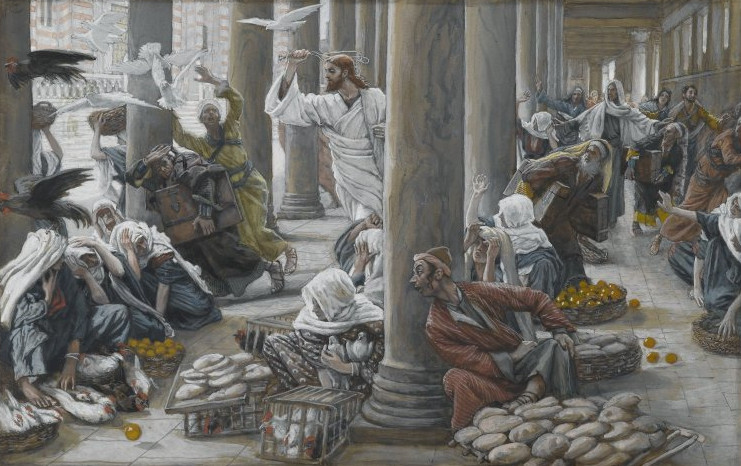
\includegraphics[width=\textwidth]{cleansing-temple}\label{fig:cleansing-temple}

% https://commons.wikimedia.org/wiki/File:Brooklyn_Museum_-_The_Merchants_Chased_from_the_Temple_(Les_vendeurs_chass%C3%A9s_du_Temple)_-_James_Tissot.jpg

\hfill

The purpose of this document is to construct, for my own study, a life of Jesus with a single narrative
thread, comprised mainly of a backbone of text from contemporary sources such as the gospels,
Josephus, and Tacitus \note{about-this-doc}.

\hfill B.~Crowell, 2021

\pagebreak

\tableofcontents

\pagebreak

\begin{section}{Timeline}

\subhead{Political timeline:}

ca.~72-4 BCE --- Herod the Great is king of Judea, with Rome as his patron. He renovates the Temple.

ca. 4 BCE-39 CE --- Judea is ruled by tetrarchs and an ethnarch, including Herod Antipater (``Antipas'') over Galilee.
      In 34-36 CE, Antipas loses a war with Aretas IV of Nabatea, an Arab trading empire centered on modern Jordan.

41-44 CE --- Herod Agrippa reigns over a reunified Judea. He engages in Roman power politics, sticks up for the Jews,
      and persecutes the early Christians, imprisoning Peter.

66-73 --- First Jewish–Roman War. The temple in Jerusalem is destroyed.

\subhead{Religious timeline (all dates approximate):}

4 BCE -- Jesus born.

30 CE -- John the Baptist executed.

30 CE -- Jesus crucified.

53 CE -- 1 Corinthians written.

65 CE -- James, brother of Jesus, martyred. Paul and Peter martyred.

70 CE -- Gospel of Mark written.

90 CE -- Luke/Acts written.

\end{section}

\vfill

\pagebreak

\fig{john-in-the-wilderness}

\begin{section}{John the Baptist}\index{John the Baptist}

\comm{The Gospel of Mark is likely the first written biographical material about Jesus,\footnote{The Pauline epistles were probably 10-20 years
earlier, but assume their audience is already familiar with the gospels.}
and it begins not with a description of Jesus but of John the Baptist.
We know nothing reliable about John's birthplace or date of birth. Luke, in the course of a miraculous birth story, claims that
John came from a priestly family:}



\luke{1:5}{There was in the days of Herod, the king of Judea, a certain priest named Zacharias [John's father], of the priestly division of Abijah.}

\comm{
John was a great celebrity of his time and place, meriting a long passage in
Josephus (much longer than the brief mention of Jesus\footnote{Antiquities of the Jews 20-9;
excluding the likely forgery in 18-3}).
Josephus says:\footnote{Antiquities 18-5-2} % https://www.gutenberg.org/files/2848/2848-h/2848-h.htm#link182HCH0005
}\index{Josephus}

\begin{quotetext}\index[texts]{Josephus}\label{josephus-baptism}
Now some of the Jews thought that the destruction of Herod [Antipater]'s army [ca.~36 CE, by the Nabateans] came
from God, and that very justly, as a punishment of what he did against
John, that was called the Baptist: for Herod slew him, who was a good
man, and commanded the Jews to exercise virtue, both as to
righteousness towards one another, and piety towards God, and so to
come to baptism; for that the washing [with water] would be acceptable
to him, if they made use of it, not in order to the putting away [or
the remission] of some sins [only], but for the purification of the
body; supposing still that the soul was thoroughly purified beforehand
by righteousness.
\end{quotetext}

\comm{\index{baptism}{John the Baptist!baptism rite}
Josephus's description of the significance of the baptism ritual is probably
distorted and sanitized in order to compromise between John's popularity and Josephus's sympathies
with the Roman-Jewish regime. Mark gives a different description: --
}

\gospelmark{1:4}{John came baptizing in the wilderness and preaching the
baptism of repentance for forgiveness of sins.  All the country of
Judea and all those of Jerusalem went out to him. They were baptized
by him in the Jordan river, confessing their sins.}

\comm{
John's actions and the symbolism of the Jordan were extremely politically provocative both to Rome and to
to the Judean client regime and its centralized theocracy at the temple in Jerusalem.\note{john-provocative}.
}

\comm{
Mark describes John as an ascetic:\note{john-ascetic}
}

\gospelmark{1:6}{John was clothed with camel’s hair and a leather belt around his waist. He ate locusts
and wild honey.}


\comm{
Matthew, unlike Mark, has John prefiguring Jesus's mission by saying
in addition,
}

\matthew{3:2}{``Repent, for the Kingdom of Heaven is at hand!''}

\comm{
and hurling abuse directly in the face of the priestly class as a ``brood of vipers'' (3:7). We don't
know whether John's message was actually apocalyptic or so explicitly antiestablishment.

Luke recounts further social teachings of John (likely inauthentic \note{john-social}):
}

\luke{3:10}{The multitudes asked him, ``What then must we do?''
 He answered them, ``He who has two coats, let him give to him who has none. He who has food, let him do likewise.''
 Tax collectors also came to be baptized, and they said to him, ``Teacher, what must we do?''
 He said to them, ``Collect no more than that which is appointed to you.''
 Soldiers also asked him, saying, ``What about us? What must we do?''
He said to them, ``Extort from no one by violence, neither accuse anyone wrongfully. Be content with your wages.''}

\comm{
Josephus continues with the story of John's doom:
}\index{John the Baptist!death}\label{john-the-baptist-death}

\begin{quotetext}\index[texts]{Josephus}
Now when [many] others came in crowds about him, for
they were very greatly moved [or pleased] by hearing his words, Herod,
who feared lest the great influence John had over the people might put
it into his power and inclination to raise a rebellion, [for they
seemed ready to do any thing he should advise,] thought it best, by
putting him to death, to prevent any mischief he might cause, and not
bring himself into difficulties, by sparing a man who might make him
repent of it when it would be too late. Accordingly he was sent a
prisoner, out of Herod's suspicious temper, to Macherus, the castle I
before mentioned, and was there put to death [around 30 CE]. Now the Jews had an
opinion that the destruction of this army was sent as a punishment
upon Herod, and a mark of God's displeasure to him.
\end{quotetext}

\comm{
John was believed by some to have been the messiah, and he retained a body of followers for
generations after his death.
}


\end{section}

\begin{section}{Jesus's origins and early life}

\comm{
Mark, John, and Paul ignore the question of Jesus's birth.\footnote{Luke and Matthew provide stories of a miraculous birth,
along with a ``massacre of the innocents'' (Matthew 2:16).} Embedded in the miraculous birth stories is the statement
that he is an oldest son, born (ca.~4 BCE) in
very humble circumstances.
}

\luke{2:7}{[Mary] gave birth to her firstborn son. She wrapped him in bands of cloth and laid him in a manger\ldots}\index{Mary}

\comm{
The skeptical Nazareans later scornfully recount the background of this uppity local boy (\note{family-interp}):
}

\gospelmark{6:2}{``What is the wisdom that is given to this man, that such
mighty works come about by his hands? Isn’t this the manual laborer, the
son of Mary and brother of James, Joses, Judah, and Simon? Aren’t his
sisters here with us?'' So they were offended at him.}

\comm{
Josephus (Antiquities 20-9-1) confirms that Jesus has a brother James, who was later to become the movement's main leader
in Jerusalem \note{james}:\index{James, brother of Jesus}
}

\begin{quotetext} % https://www.gutenberg.org/files/2848/2848-h/2848-h.htm#link202HCH0009
\ldots [the procurator Albinus] assembled the sanhedrim of judges, and brought before them the brother of Jesus, who was called Christ, whose name was James, and some others \ldots [and] delivered them to be stoned
\end{quotetext}

\comm{
Jesus grew up in the tiny village of Nazareth, in Galilee,\note{jesus-galilee} speaking Aramaic.\note{jesus-aramaic}
He probably never learned to read, but he must have had an opportunity
at least to hear an oral Aramaic version (targum) of the Jewish Bible and learn it thoroughly \note{literacy}.\index{Nazareth}

 At periodic festivals,
Jews who were able to afford to travel gathered in great crowds at the temple in
Jerusalem:
}

\luke{2:41}{His parents went every year to Jeru\-salem at the feast of the Passover.  When he was twelve years old, they went up to Jerusalem according to the custom of the feast;  and when they had fulfilled the days, as they were returning, the boy Jesus stayed behind in Jerusalem. Joseph and his mother didn’t know it,  but supposing him to be in the company, they went a day’s journey; and they looked for him among their relatives and acquaintances.  When they didn’t find him, they returned to Jerusalem, looking for him.  After three days they found him in the temple, sitting in the middle of the teachers, both listening to them and asking them questions.  All who heard him were amazed at his understanding and his answers.  When they saw him, they were astonished; and his mother said to him, ``Son, why have you treated us this way? Behold, your father and I were anxiously looking for you.''
 He said to them, ``Why were you looking for me? Didn’t you know that I must be in my Father’s house?''}

\comm{
This miracle story may preserve a factual picture of a precocious child getting an education against all odds, or
it may be that Jesus gained his education as a teenager or an adult, like Frederick Douglass. The gospels leap
over Jesus's youth and young adulthood to ca.~28 CE, when Jesus would have been about 31.
}

\luke{3:1}{Now in the fifteenth year of the reign [14-37 CE] of Tiberius
Caesar\ldots the word of God came to John, the son of Zacharias, in
the wilderness.  He came into all the region around the Jordan,
preaching the baptism of repentance for remission of sins.}

\comm{
Among John's followers were a number of people who were later to become the early Christians.
One of the few things we can know securely about the historical Jesus is that he was baptized
by John:
}

\gospelmark{1:9}{In those days, Jesus came from Nazareth of Galilee, and was baptized by John in the Jordan.}\index{baptism!of Jesus by John}

\comm{Others include Simon Peter, apostle and founder of the Church (p.~\pageref{peter-called}), and his brother, the apostle Andrew (John 1:40);
 as well as more who are described in Acts:}\index{John the Baptist!followers}

\bible{Acts 19:1}{While Apollos [an Alexandrian Jew who was a follower of John and then converted in Acts 18] was at Corinth, Paul, having passed through the upper country, came to Ephesus and found certain disciples. He said to them, “Did you receive the Holy Spirit when you believed?”
They said to him, ``No, we haven’t even heard that there is a Holy Spirit.''
 He said, ``Into what then were you baptized?''
They said, ``Into John’s baptism.''
 Paul said, ``John indeed baptized with the baptism of repentance, saying to the people that they should believe in the one who would come after him, that is, in Christ Jesus.''
 When they heard this, they were baptized in the name of the Lord Jesus.}

\luke{3:18}{Then with many other exhortations [John] preached good news to the people, but Herod the tetrarch, being reproved by him for Herodias, his brother’s wife, and for all the evil things which Herod had done, added this also to them all, that he shut up John in prison.}

\gospelmark{1:12}{Immediately the Spirit drove [Jesus] out into the
wilderness. He was there in the wild\-erness forty days, tempted by
Satan. He was with the wild animals; and the angels were serving him.\footnote{\reftex{Luke 4} has a lengthier account of
the temptation, with the devil offering Jesus worldly power. \personal{This is unlikely to have any connection to
Jesus's actual visions and spiritual experiences. It sounds more like the later sanitizing of the early
Christian religion for consumption by Romans, who did not want to be part of a religion that preached the overthrow
of the empire.}}}
\end{section}\index{temptation of Christ|see{wilderness, Jesus in}}\index{wilderness, Jesus in}

\fig{jesus-in-wilderness}

\begin{section}{Early mission and calling of the apostles}

\luke{3:23}{Jesus himself, when he began to teach, was about thirty years old\ldots}

\subhead{Preaching in Nazareth}

\gospelmark{1:14}{ Now after John was arrested, Jesus came
into Galilee, preaching the Good News of God’s Kingdom, and saying,
``The time is fulfilled, and God’s Kingdom is at hand! Repent, and
believe in the Good News.''}

\luke{4:14}{Jesus returned in the power of the Spirit into Galilee, and news about him spread through all the surrounding area. \ldots
  He came to Nazareth, where he had been brought up.\footnote{Luke has Jesus reading from a scroll and teaching about Elijah and
Isaiah. \personal{This seems like a later addition by Luke, in an effort to present Jesus as paralleling and fulfilling the prophets. The scene
is absent from Mark.}}}

\luke{4:22}{All testified about him and wondered at the gracious words which proceeded out of his mouth; and they said, ``Isn't this Joseph's son?''}

\luke{4:28}{ They were all filled with wrath in the synagogue as they heard these things.   They rose up, threw him out of the city, and led him to the brow of the hill that their city was built on, that they might throw him off the cliff.   But he, passing through the middle of them, went his way.}

\fig{fishers-of-men}

\subhead{Capernaum; The first apostles}\index{Capernaum!preaching at}\index{Peter!calling of}\index{apostles}

\gospelmark{1:16}{Passing along by the sea of Galilee,\footnote{John 1:44 says Bethsaida.\note{bethsaida}} he saw Simon
  and Andrew, the brother of Simon, casting a net into the sea, for
  they were fishermen.  Jesus said to them, ``Come after me, and I
  will make you into fishers for men.''  Immediately they left their
  nets, and followed him.  Going on a little further from there, he
  saw James the son of Zebedee, and John his brother, who were also in
  the boat mending the nets.  Immediately he called them, and they
  left their father, Zebedee, in the boat with the hired servants, and
  went after him.  They went into Capernaum, and immediately on the
  Sabbath day he entered into the synagogue and taught.  They were
  astonished at his teaching, for he taught them as having authority,
  and not as the scribes \note{jesus-writing}.}

\luke{8:1}{
[He] went about through cities and villages, preaching and bringing the good news of God's Kingdom. With him were the twelve,   and certain women who had been healed of evil spirits and infirmities: Mary who was called Magdalene, from whom seven demons had gone out;   and Joanna, the wife of Chuzas, Herod's steward; Susanna; and many others who served them from their possessions.  
}\index{Mary Magdalene}\index{Joanna}\index{Susanna}

\fig{mary-magdalene-at-the-feet-of-jesus}

\comm{
Jesus gathers male and female followers and creates his
own knock-off of John's illicit knock-off of the Temple's rites.
Where John baptized people and then sent them home, Jesus 
carries out an itinerant lifestyle ministry. 

The first four apostles are Simon Peter (\note{peter}), Andrew, John, and James the Greater. Simon Peter and Andrew
are described in \reftex{John 1:40} as having been followers of John the Baptist.\label{peter-called}\index{John (apostle)}\index{James the Greater (apostle)}
}

\gospelmark{1:23}{Immediately there was in their synagogue [in Capernaum] a man with an unclean spirit, and he cried out,   saying, ``Ha! What do we have to do with you, Jesus, you Nazarene? Have you come to destroy us? I know you who you are: the Holy One of God!''
  Jesus rebuked him, saying, ``Be quiet, and come out of him!''
  The unclean spirit, convulsing him and crying with a loud voice, came out of him.   They were all amazed, so that they questioned among themselves, saying, ``What is this? A new teaching? For with authority he commands even the unclean spirits, and they obey him!''   The report of him went out immediately everywhere into all the region of Galilee and its surrounding area.

  Immediately, when they had come out of the synagogue, they came into the house of Simon and Andrew, with James and John.
   Now Simon's wife's mother\footnote{So Simon Peter is married.} lay sick with a fever, and immediately they told him about her.   He came and took her by the hand and raised her up. The fever left her immediately, and she served them.

  At evening, when the sun had set, they brought to him all who were sick and those who were possessed by demons.   All the city was gathered together at the door.   He healed many who were sick with various diseases and cast out many demons. He didn't allow the demons to speak, because they knew him.}

\fig[0.6]{driving-out-demons}

\gospelmark{1:35}{Early in the morning, while it was still dark, he rose up and went out, and departed into a deserted place, and prayed there.   Simon and those who were with him searched for him.   They found him and told him, ``Everyone is looking for you.''
  He said to them, ``Let's go elsewhere into the next towns, that I may preach there also, because I came out for this reason.''   He went into their synagogues throughout all Galilee, preaching and casting out demons.}

\comm{
It would have been more culturally expected for a healer to set up shop in one place. Jesus doesn't do so, nor does
he accept money or pray when he heals. The reason for the secrecy and hiding is clarified in the following incident.
}

\subhead{The leper}\index{leper}\index{healing!leper}

\gospelmark{1:40}{A leper came to him, begging him, kneeling down to him, and saying to him, ``If you want to, you can make me clean.''
  Being moved with anger,\footnote{Some sources have ``compassion.''} he stretched out his hand, and touched him, and said to him, ``I want to. Be made clean.''   When he had said this, immediately the leprosy departed from him and he was made clean.   He strictly warned him and immediately sent him out,   and said to him, ``See that you say nothing to anybody, but go show yourself to the priest and offer for your cleansing the things which Moses commanded, for a testimony to them.''

  But he went out, and began to proclaim it much, and to spread about the matter, so that Jesus could no more openly enter into a city, but was outside in desert places. People came to him from everywhere. }

\comm{This scene has a seditious point that would be obvious to first-century Palestinian Jews, and this clarifies
the secrecy and hiding, as well as Jesus's initial anger (\note{leper-seditious}).}

\fig{healing-the-paralytic}

\subhead{The paralytic}\index{paralytic, healing}\index{healing!paralytic}

\gospelmark{2:1}{When he entered again into Capernaum after some days, it was heard that he was at home.   Immediately many were gathered together, so that there was no more room, not even around the door; and he spoke the word to them.   Four people came, carrying a paralytic to him.   When they could not come near to him for the crowd, they removed the roof where he was. When they had broken it up, they let down the mat that the paralytic was lying on.   Jesus, seeing their faith, said to the paralytic, ``Son, your sins are forgiven you.''

  But there were some of the scribes sitting there and reasoning in their hearts,   ``Why does this man speak blasphemies like that? Who can forgive sins but God alone?''

  Immediately Jesus, perceiving in his spirit that they so reasoned within themselves, said to them, ``Why do you reason these things in your hearts?    Which is easier, to tell the paralytic, `Your sins are forgiven;' or to say, `Arise, and take up your bed, and walk?'    
But that you may know that the Son of Man\note{son-of-man} 
has authority\footnote{The issue of authority, implicit in the story of the leper, is here made explicit.}
on earth to forgive sins''--he said to the paralytic--    ``I tell you, arise, take up your mat, and go to your house.'' 

He arose, and immediately took up the mat and went out in front of them all, so that they were all amazed and glorified God, saying, ``We never saw anything like this!''}

\comm{In \reftex{John 2:1-11}, Jesus turns water in to wine at the wedding at Cana.}\index{Cana!wedding at}

\subhead{Calling Matthew}\index{Matthew (apostle)}

\gospelmark{2:13}{He went out again by the seaside. All the multitude came to him, and he taught them.   As he passed by, he saw 
[Matthew\footnote{The apostle. Named in Mark as Levi the son of Alphaeus.}] sitting at the tax office.\footnote{Tax collectors were hated
both because the taxes were exorbitant and because the taxes were being collected for the Romans.}
He said to him, ``Follow me.'' And he arose and followed him.}

\gospelmark{3:7}{
  Jesus withdrew to the sea with his disciples; and a great multitude followed him from Galilee, from Judea,   from Jerusalem, from Idumaea, beyond the Jordan, and those from around Tyre and Sidon. A great multitude, hearing what great things he did, came to him.   He said to his disciples that a little boat should stay near him because of the crowd, so that they wouldn't press on him.   For he had healed many, so that as many as had diseases pressed on him that they might touch him.   The unclean spirits, whenever they saw him, fell down before him and cried, ``You are the Son of God!''   He sternly warned them that they should not make him known.
}

\subhead{The commissioning of the apostles}\index{apostles!commissioning}

\comm{
John the Baptist never deputizes anyone to act on his behalf, but Jesus does:
}

\gospelmark{3:13}{
  He went up into the mountain and called to himself those whom he wanted, and they went to him.   He appointed twelve, that they might be with him, and that he might send them out to preach   and to have authority to heal sicknesses and to cast out demons:   Simon (to whom he gave the name Peter);   James the son of Zebedee; and John, the brother of James (whom he called Boanerges, which means, Sons of Thunder);   Andrew; Philip; Bartholomew; Matthew; Thomas; James, the son of Alphaeus; Thaddaeus; Simon the Zealot;   and Judas Iscariot, who also betrayed him.\index{apostles!list}
}

\comm{Jesus reassures the apostles: \note{matthew-second-discourse}}

\matthew{10:16}{
 ``Behold, I send you out as sheep among wolves. Therefore be wise as serpents and harmless as doves.''
}

\matthew{10:26}{
``Therefore don’t be afraid of them, for there is nothing covered that will not be revealed, or hidden that will not be known.''
}

\matthew{10:29}{
``Aren't two sparrows sold for a penny? Not one of them falls to the ground apart from your Father's will.    But the very hairs of your head are all numbered.    Therefore don't be afraid. You are of more value than many sparrows.''
}\index{sparrows}

\comm{But:}

\matthew{10:34}{\note{not-peace-but-a-sword}
``Don't think that I came to send peace on the earth. I didn't come to send peace, but a sword.    For I came to set a man at odds against his father, and a daughter against her mother, and a daughter-in-law against her mother-in-law.    A man's foes will be those of his own household.''
}\index{peace!not peace but a sword}

\end{section}

\fig[0.75]{meal-in-house-of-matthew}

\begin{section}{Sinners, tax collectors, and gentiles}\index{sinners}\index{tax collectors}
\subhead{Eating with sinners; parables; foraging on the sabbath}

\gospelmark{2:15}{  He was reclining at the table in his house, and many tax collectors and sinners sat down with Jesus and his disciples, for there were many, and they followed him.   The scribes and the Pharisees, when they saw that he was eating with the sinners and tax collectors, said to his disciples, ``Why is it that he eats and drinks with tax collectors and sinners?''

  When Jesus heard it, he said to them, ``Those who are healthy have no need for a physician, but those who are sick. I came not to call the righteous, but sinners to repentance.''}

\subhead{Parable of the lost sheep}\index{lost sheep (parable)}

\luke{15:1}{Now all the tax collectors and sinners were coming close to him to hear him.   The Pharisees and the scribes murmured, saying, ``This man welcomes sinners, and eats with them.''

  He told them this parable:    ``Which of you men, if you had one hundred sheep and lost one of them, wouldn't leave the ninety-nine in the wilderness and go after the one that was lost, until he found it?    When he has found it, he carries it on his shoulders, rejoicing.    When he comes home, he calls together his friends and his neighbors, saying to them, `Rejoice with me, for I have found my sheep which was lost!'\footnote{Luke
finishes by making the allegory explicit, then in 15:8 follows up
with a second, closely parallel parable about a lost coin.}
}

\subhead{Parable of the prodigal son}\index{prodigal son (parable)}

\luke{15:11}{
  He said, ``A certain man had two sons.    The younger of them said to his father, `Father, give me my share of your property.' So he divided his livelihood between them.    Not many days after, the younger son gathered all of this together and traveled into a far country. There he wasted his property with riotous living.    When he had spent all of it, there arose a severe famine in that country, and he began to be in need.    He went and joined himself to one of the citizens of that country, and he sent him into his fields to feed pigs.    He wanted to fill his belly with the pods that the pigs ate, but no one gave him any.    But when he came to himself, he said, `How many hired servants of my father's have bread enough to spare, and I'm dying with hunger!    I will get up and go to my father, and will tell him, ``Father, I have sinned against heaven and in your sight.    I am no more worthy to be called your son. Make me as one of your hired servants.'' '

   ``He arose and came to his father. But while he was still far off, his father saw him and was moved with compassion, and ran, fell on his neck, and kissed him.    The son said to him, `Father, I have sinned against heaven and in your sight. I am no longer worthy to be called your son.'

   ``But the father said to his servants, `Bring out the best robe and put it on him. Put a ring on his hand and sandals on his feet.    Bring the fattened calf, kill it, and let's eat and celebrate;    for this, my son, was dead and is alive again. He was lost and is found.' Then they began to celebrate.

   ``Now his elder son was in the field. As he came near to the house, he heard music and dancing.    He called one of the servants to him and asked what was going on.    He said to him, `Your brother has come, and your father has killed the fattened calf, because he has received him back safe and healthy.'    But he was angry and would not go in. Therefore his father came out and begged him.    But he answered his father, `Behold, these many years I have served you, and I never disobeyed a commandment of yours, but you never gave me a goat, that I might celebrate with my friends.    But when this your son came, who has devoured your living with prostitutes, you killed the fattened calf for him.'

   ``He said to him, `Son, you are always with me, and all that is mine is yours.    But it was appropriate to celebrate and be glad, for this, your brother, was dead, and is alive again. He was lost, and is found.' '' 
}

\subhead{Parable of the bridegroom}\index{bridegroom (parable)}

\gospelmark{2:18}{John's disciples and the Pharisees were fasting, and they came and asked him, ``Why do John's disciples and the disciples of the Pharisees fast, but your disciples don't fast?''

  Jesus said to them, ``Can the groomsmen fast while the bridegroom is with them? As long as they have the bridegroom with them, they can't fast.    But the days will come when the bridegroom will be taken away from them, and then they will fast.

    No one sews a piece of unshrunk cloth on an old garment, or else the patch shrinks and the new tears away from the old, and a worse hole is made.    No one puts new wine into old wineskins; or else the new wine will burst the skins, and the wine pours out, and the skins will be destroyed; but they put new wine into fresh wineskins.'' }

\comm{
John was an ascetic;
Jesus rejects John's asceticism, but retains an antimaterialist slant.
}

\fig{plucking-corn-on-the-sabbath}

\subhead{Foraging on the sabbath}\index{sabbath!foraging on}

\gospelmark{2:23}{He was going on the Sabbath day through the grain fields; and his disciples began, as they went, to pluck the ears of grain.   The Pharisees said to him, ``Behold, why do they do that which is not lawful on the Sabbath day?''

  He said to them, ``Did you never read what David did when he had need and was hungry--he, and those who were with him?    How he entered into God's house at the time of Abiathar the high priest, and ate the show bread, which is not lawful to eat except for the priests, and gave also to those who were with him?''

  He said to them, ``The Sabbath was made for man, not man for the Sabbath.    Therefore the Son of Man is lord even of the Sabbath.'' 
}


\subhead{The withered hand}\index{withered hand (healing)}

\gospelmark{3:1}{
He entered again into the synagogue, and there was a man there whose hand was withered.   They watched him, whether he would heal him on the Sabbath day, that they might accuse him.   He said to the man whose hand was withered, ``Stand up.''   He said to them, ``Is it lawful on the Sabbath day to do good or to do harm? To save a life or to kill?'' But they were silent.   When he had looked around at them with anger, being grieved at the hardening of their hearts, he said to the man, ``Stretch out your hand.'' He stretched it out, and his hand was restored as healthy as the other.   The Pharisees went out, and immediately conspired with the Herodians against him, how they might destroy him.}

\fig[1]{good-samaritan}\index{Samaritan, good}

\subhead{Who is my neighbor?; the good Samaritan}\label{good-samaritan}

\luke{10:25}{\footnote{The theme is reiterated with another Samaritan in \reftex{Luke 17:14}.}
Behold, a certain lawyer stood up and tested him, saying, ``Teacher, what shall I do to inherit eternal life?''

  He said to him, ``What is written in the law? How do you read it?''

  He answered, ``You shall love the Lord your God with all your heart, with all your soul, with all your strength, and with all your mind; and your neighbor as yourself.''

  He said to him, ``You have answered correctly. Do this, and you will live.''

  But he, desiring to justify himself, asked Jesus, ``Who is my neighbor?''

  Jesus answered, ``A certain man was going down from Jerusalem to Jericho, and he fell among robbers, who both stripped him and beat him, and departed, leaving him half dead.    By chance a certain priest was going down that way. When he saw him, he passed by on the other side.    In the same way a Levite also, when he came to the place and saw him, passed by on the other side.    But a certain Samaritan, as he traveled, came where he was. When he saw him, he was moved with compassion,    came to him, and bound up his wounds, pouring on oil and wine. He set him on his own animal, brought him to an inn, and took care of him.    On the next day, when he departed, he took out two denarii, gave them to the host, and said to him, `Take care of him. Whatever you spend beyond that, I will repay you when I return.'    Now which of these three do you think seemed to be a neighbor to him who fell among the robbers?''

  He said, ``He who showed mercy on him.''
Then Jesus said to him, ``Go and do likewise.'' 
}

\comm{The point of the story is not just to be nice to strangers who are in distress.
It criticizes the priesthood of the temple in Jerusalem in the strongest possible terms, by comparing them
unfavorably with an ethnic group, the Samaritans, who are hated by the Jews. It also shows that Jesus's mission,
and his ethics, transcend ethnic boundaries --  a radical break with material in the Hebrew Bible
such as the Book of Esther.
Compare with ``Who are my mother and my brothers?,'' p.~\pageref{who-are-my-mother-and-my-brothers}.}

\end{section}

\begin{section}{The sermon on the mount}\index{sermon on the mount}

\comm{
Matthew 5-7 is the sermon on the mount, the greatest statement of Christian ethics.\note{sermon-on-the-mount} 
Its contents are completely different from the rest of the gospels, which are concerned entirely
with the coming end of the world.\note{new-ethics}
Jesus set a moral example in his itinerant lifestyle ministry, but his conduct is sometimes inconsistent with
the wisdom sayings presented in this sermon.\note{jesus-ethics-conduct}
I've left out some verses argued by Geza Vermes to be inauthentic. % https://www.sermononthemount.org.uk/Background/Authenticity.html
}

\matthew{5:1}{
Seeing the multitudes, he went up onto the mountain. When he had sat down, his disciples came to him. He opened his mouth and taught them, saying, 
}

\subhead{The beatitudes}\index{beatitudes}

\matthew{5:3}{
``Blessed are the poor in spirit,
for theirs is the Kingdom of Heaven.

   Blessed are those who mourn,
for they shall be comforted.

   Blessed are the gentle,
for they shall inherit the earth.

   Blessed are those who hunger and thirst for righteousness,
for they shall be filled.

   Blessed are the merciful,
for they shall obtain mercy.

   Blessed are the pure in heart,
for they shall see God.

   Blessed are the peacemakers,
for they shall be called children of God.

   Blessed are those who have been persecuted for righteousness' sake,
for theirs is the Kingdom of Heaven.\footnote{5:11 about persecution is likely a later addition, since the persecution of Christians
hasn't happened yet.}
}

\matthew{5:12}{
Rejoice, and be exceedingly glad, for great is your reward in heaven. [\ldots]
}

\matthew{5:13}{
You are the salt of the earth, but if the salt has lost its flavor, with what will it be salted? It is then good for nothing, but to be cast out and trodden under the feet of men.
}\index{salt of the earth}

\matthew{5:14}{You are the light of the world. A city  on a hill can't be hidden.    Neither do you light a lamp and put it under a measuring basket, but on a stand; and it shines to all who are in the house.    Even so, let your light shine before men, that they may see your good works and glorify your Father who is in heaven.\footnote{5:14-15 is a preview of 9:49.}}\index{city on a hill (parable)}\index{lamp (parable)}

\subhead{Extending the Mosaic law}

\matthew{5:17}{
``Don't think that I came to destroy the law or the prophets. I didn't come to destroy, but to fulfill.    For most certainly, I tell you, until heaven and earth pass away, not even one smallest letter or one tiny pen stroke shall in any way pass away from the law, until all things are accomplished.    Therefore, whoever shall break one of these least commandments and teach others to do so, shall be called least in the Kingdom of Heaven; but whoever shall do and teach them shall be called great in the Kingdom of Heaven.    For I tell you that unless your righteousness exceeds that of the scribes and Pharisees, there is no way you will enter into the Kingdom of Heaven.

   ``You have heard that it was said to the ancient ones, `You shall not murder;' and `Whoever murders will be in danger of the judgment.'    But I tell you that everyone who is angry with his brother without a cause  will be in danger of the judgment. Whoever says to his brother, `Raca!' will be in danger of the council. Whoever says, `You fool!' will be in danger of the fire of Gehenna.

   ``If therefore you are offering your gift at the altar, and there remember that your brother has anything against you,    leave your gift there before the altar, and go your way. First be reconciled to your brother, and then come and offer your gift.    Agree with your adversary quickly while you are with him on the way; lest perhaps the prosecutor deliver you to the judge, and the judge deliver you to the officer, and you be cast into prison.    Most certainly I tell you, you shall by no means get out of there until you have paid the last penny.

   ``You have heard that it was said,  `You shall not commit adultery;'    but I tell you that everyone who gazes at a woman to lust after her has committed adultery with her already in his heart.    If your right eye causes you to stumble, pluck it out and throw it away from you. For it is more profitable for you that one of your members should perish than for your whole body to be cast into Gehenna.    If your right hand causes you to stumble, cut it off, and throw it away from you. For it is more profitable for you that one of your members should perish, than for your whole body to be cast into Gehenna.

   ``It was also said, `Whoever shall put away his wife, let him give her a writing of divorce,'    but I tell you that whoever puts away his wife, except for the cause of sexual immorality, makes her an adulteress; and whoever marries her when she is put away commits adultery.

   ``Again you have heard that it was said to the ancient ones, `You shall not make false vows, but shall perform to the Lord your vows,'    but I tell you, don't swear at all: neither by heaven, for it is the throne of God;    nor by the earth, for it is the footstool of his feet; nor by Jerusalem, for it is the city of the great King.    Neither shall you swear by your head, for you can't make one hair white or black.    But let your `Yes' be `Yes' and your `No' be `No.' Whatever is more than these is of the evil one.

   ``You have heard that it was said, `An eye for an eye, and a tooth for a tooth.'    But I tell you, don't resist him who is evil; but whoever strikes you on your right cheek, turn to him the other also.    If anyone sues you to take away your coat, let him have your cloak also.    Whoever compels you to go one mile, go with him two.    Give to him who asks you, and don't turn away him who desires to borrow from you.

   ``You have heard that it was said, `You shall love your neighbor  and hate your enemy.'    But I tell you, love your enemies, bless those who curse you, do good to those who hate you, and pray for those who mistreat you and persecute you,    that you may be children of your Father who is in heaven. For he makes his sun to rise on the evil and the good, and sends rain on the just and the unjust.    For if you love those who love you, what reward do you have? Don't even the tax collectors do the same?    If you only greet your friends, what more do you do than others? Don't even the tax collectors do the same?    Therefore you shall be perfect, just as your Father in heaven is perfect.
}

\subhead{Prayer}

\matthew{6:1}{
    ``Be careful that you don't do your charitable giving before men, to be seen by them, or else you have no reward from your Father who is in heaven.    Therefore, when you do merciful deeds, don't sound a trumpet before yourself, as the hypocrites do in the synagogues and in the streets, that they may get glory from men. Most certainly I tell you, they have received their reward.    But when you do merciful deeds, don't let your left hand know what your right hand does,    so that your merciful deeds may be in secret, then your Father who sees in secret will reward you openly.

   ``When you pray, you shall not be as the hypocrites, for they love to stand and pray in the synagogues and in the corners of the streets, that they may be seen by men. Most certainly, I tell you, they have received their reward.    But you, when you pray, enter into your inner room, and having shut your door, pray to your Father who is in secret; and your Father who sees in secret will reward you openly.    In praying, don't use vain repetitions as the Gentiles do; for they think that they will be heard for their much speaking.    Therefore don't be like them, for your Father knows what things you need before you ask him.    Pray like this:
}

\matthew{6:9}{\index{Lord's prayer}
`` `Our Father in heaven, may your name be kept holy.

   Let your Kingdom come.
Let your will be done on earth as it is in heaven.

   Give us today our daily bread.

   Forgive us our debts,
as we also forgive our debtors.

   Bring us not into temptation,
but deliver us from the evil one.

For yours is the Kingdom, the power, and the glory forever. Amen.'
}

\matthew{6:14}{
   ``For if you forgive men their trespasses, your heavenly Father will also forgive you.    But if you don't forgive men their trespasses, neither will your Father forgive your trespasses.

   ``Moreover when you fast, don't be like the hypocrites, with sad faces. For they disfigure their faces that they may be seen by men to be fasting. Most certainly I tell you, they have received their reward.    But you, when you fast, anoint your head and wash your face,    so that you are not seen by men to be fasting, but by your Father who is in secret; and your Father, who sees in secret, will reward you.}

\fig{mammon}

\subhead{Antimaterialism}\index{matrialism}

\matthew{6:19}{
   ``Don't lay up treasures for yourselves on the earth, where moth and rust consume, and where thieves break through and steal;    but lay up for yourselves treasures in heaven, where neither moth nor rust consume, and where thieves don't break through and steal;    for where your treasure is, there your heart will be also.

   ``The lamp of the body is the eye. If therefore your eye is sound, your whole body will be full of light.    But if your eye is evil, your whole body will be full of darkness. If therefore the light that is in you is darkness, how great is the darkness!

   ``No one can serve two masters, for either he will hate the one and love the other, or else he will be devoted to one and despise the other. You can't serve both God and Mammon.    Therefore I tell you, don't be anxious about your life: what you will eat, or what you will drink; nor yet for your body, what you will wear. Isn't life more than food, and the body more than clothing?    See the birds of the sky, that they don't sow, neither do they reap, nor gather into barns. Your heavenly Father feeds them. Aren't you of much more value than they?

   ``Which of you by being anxious, can add one moment to his lifespan?    Why are you anxious about clothing? Consider the lilies of the field, how they grow. They don't toil, neither do they spin,    yet I tell you that even Solomon in all his glory was not dressed like one of these.    But if God so clothes the grass of the field, which today exists and tomorrow is thrown into the oven, won't he much more clothe you, you of little faith?

   ``Therefore don't be anxious, saying, `What will we eat?', `What will we drink?' or, `What will we wear?'    For the Gentiles seek after all these things; for your heavenly Father knows that you need all these things.    But seek first God's Kingdom and his righteousness; and all these things will be given to you as well.    Therefore don't be anxious for tomorrow, for tomorrow will be anxious for itself. Each day's own evil is sufficient. 
}

\subhead{Don't judge}\index{judging others}

\matthew{7:1}{
    ``Don't judge, so that you won't be judged.    For with whatever judgment you judge, you will be judged; and with whatever measure you measure, it will be measured to you.    Why do you see the speck that is in your brother's eye, but don't consider the beam that is in your own eye?    Or how will you tell your brother, `Let me remove the speck from your eye,' and behold, the beam is in your own eye?    You hypocrite! First remove the beam out of your own eye, and then you can see clearly to remove the speck out of your brother's eye.

\subhead{Wisdom sayings}

   ``Don't give that which is holy to the dogs, neither throw your pearls before the pigs, lest perhaps they trample them under their feet, and turn and tear you to pieces.

   ``Ask, and it will be given you. Seek, and you will find. Knock, and it will be opened for you.    For everyone who asks receives. He who seeks finds. To him who knocks it will be opened.    Or who is there among you who, if his son asks him for bread, will give him a stone?    Or if he asks for a fish, who will give him a serpent?    If you then, being evil, know how to give good gifts to your children, how much more will your Father who is in heaven give good things to those who ask him!    Therefore, whatever you desire for men to do to you, you shall also do to them; for this is the law and the prophets.

   ``Enter in by the narrow gate; for the gate is wide and the way is broad that leads to destruction, and there are many who enter in by it.    How narrow is the gate and the way is restricted that leads to life! There are few who find it.

   ``Beware of false prophets, who come to you in sheep's clothing, but inwardly are ravening wolves.    By their fruits you will know them. Do you gather grapes from thorns or figs from thistles?    Even so, every good tree produces good fruit, but the corrupt tree produces evil fruit.    A good tree can't produce evil fruit, neither can a corrupt tree produce good fruit.    Every tree that doesn't grow good fruit is cut down and thrown into the fire.    Therefore by their fruits you will know them.

   ``Not everyone who says to me, `Lord, Lord,' will enter into the Kingdom of 
Heaven,\footnote{Contradicted by Paul in Romans 10:13, ``Whoever will call on the name of the Lord will be saved''
(quoting Joel 2:32, which refers to salvation from a plague of locusts).} but he who does the will of my Father who is in heaven.
}

\matthew{7:24}{
  ``Everyone therefore who hears these words of mine and does them, I will liken him to a wise man who built his house on a rock.    The rain came down, the floods came, and the winds blew and beat on that house; and it didn't fall, for it was founded on the rock.    Everyone who hears these words of mine and doesn't do them will be like a foolish man who built his house on the sand.    The rain came down, the floods came, and the winds blew and beat on that house; and it fell--and its fall was great.''
}

\matthew{7:28}{
  When Jesus had finished saying these things, the multitudes were astonished at his teaching,   for he taught them with authority, and not like the scribes.
}

\end{section}


\begin{section}{The kingdom of God}\index{kingdom of God}
\gospelmark{3:19}{
Then [after the commissioning of the apostles] he came into a house.   The multitude came together again, so that they could not so much as eat bread.   When his friends heard it, they went out to seize him; for they said, ``He is insane.''   The scribes who came down from Jerusalem said, ``He has Beelzebul,'' and, ``By the prince of the demons he casts out the demons.''

  He summoned them and said to them in parables, ``How can Satan cast out Satan?    If a kingdom is divided against itself, that kingdom cannot stand.    If a house is divided against itself, that house cannot stand.    If Satan has risen up against himself, and is divided, he can't stand, but has an end.    But no one can enter into the house of the strong man to plunder unless he first binds the strong man; then he will plunder his house.

   ``Most certainly I tell you, all sins of the descendants of man will be forgiven, including their blasphemies with which they may blaspheme;    but whoever may blaspheme against the Holy Spirit never has forgiveness, but is subject to eternal condemnation.''   --because they said, ``He has an unclean spirit.''\label{how-can-satan}
}

\comm{For Mark 3:31, ``Who are my mother and my brothers?,'' see p.~\pageref{who-are-my-mother-and-my-brothers}.}

\fig{sower}

\subhead{Parable of the sower}\index{sower (parable)}

\gospelmark{4:1}{
   Again he began to teach by the seaside. A great multitude was gathered to him, so that he entered into a boat in the sea and sat down. All the multitude were on the land by the sea.   He taught them many things in parables, and told them in his teaching,    ``Listen! Behold, the farmer went out to sow.    As he sowed, some seed fell by the road, and the birds came and devoured it.    Others fell on the rocky ground, where it had little soil, and immediately it sprang up, because it had no depth of soil.    When the sun had risen, it was scorched; and because it had no root, it withered away.    Others fell among the thorns, and the thorns grew up and choked it, and it yielded no fruit.    Others fell into the good ground and yielded fruit, growing up and increasing. Some produced thirty times, some sixty times, and some one hundred times as much.''   He said, ``Whoever has ears to hear, let him hear.''

  When he was alone, those who were around him with the twelve asked him about the parables.   He said to them, ``To you is given the mystery of God's Kingdom, but to those who are outside, all things are done in parables,    that `seeing they may see and not perceive, and hearing they may hear and not understand, lest perhaps they should turn again, and their sins should be forgiven them.' ''

  He said to them, ``Don't you understand this parable? How will you understand all of the parables?    The farmer sows the word.    The ones by the road are the ones where the word is sown; and when they have heard, immediately Satan comes and takes away the word which has been sown in them.    These in the same way are those who are sown on the rocky places, who, when they have heard the word, immediately receive it with joy.    They have no root in themselves, but are short-lived. When oppression or persecution arises because of the word, immediately they stumble.    Others are those who are sown among the thorns. These are those who have heard the word,    and the cares of this age, and the deceitfulness of riches, and the lusts of other things entering in choke the word, and it becomes unfruitful.    Those which were sown on the good ground are those who hear the word, accept it, and bear fruit, some thirty times, some sixty times, and some one hundred times.''}

% Omit recap of the lamp, which was already in the sermon on the mount.

\gospelmark{4:24}{
  He said to them, ``Take heed what you hear. With whatever measure you measure, it will be measured to you; and more will be given to you who hear.    For whoever has, to him more will be given; and he who doesn't have, even that which he has will be taken away from him.''

  He said, ``God's Kingdom is as if a man should cast seed on the earth,    and should sleep and rise night and day, and the seed should spring up and grow, though he doesn't know how.    For the earth bears fruit by itself: first the blade, then the ear, then the full grain in the ear.    But when the fruit is ripe, immediately he puts in the sickle, because the harvest has come.''

  He said, ``How will we liken God's Kingdom? Or with what parable will we illustrate it?    It's like a grain of mustard seed, which, when it is sown in the earth, though it is less than all the seeds that are on the earth,    yet when it is sown, grows up and becomes greater than all the herbs, and puts out great branches, so that the birds of the sky can lodge under its shadow.''

  With many such parables he spoke the word to them, as they were able to hear it.   Without a parable he didn't speak to them; but privately to his own disciples he explained everything.

  On that day, when evening had come, he said to them, ``Let's go over to the other side.''   Leaving the multitude, they took him with them, even as he was, in the boat. Other small boats were also with him.   A big wind storm arose, and the waves beat into the boat, so much that the boat was already filled.   He himself was in the stern, asleep on the cushion; and they woke him up and asked him, ``Teacher, don't you care that we are dying?''

  He awoke and rebuked the wind, and said to the sea, ``Peace! Be still!'' The wind ceased and there was a great calm.   He said to them, ``Why are you so afraid? How is it that you have no faith?''

  They were greatly afraid and said to one another, ``Who then is this, that even the wind and the sea obey him?'' 
}

\subhead{The gospel of Thomas on the kingdom of God}

\thomas{40}{
A vine has been planted without the Father -- and (as) it is not vigorous, it shall be pulled up by its roots and destroyed.\footnote{Cf.~Matthew 15:13.}
}\index{vine (parable)}

\thomas{97}{
The Sovereignty of the [Father] is like a woman who is carrying a jar full of grain. (While) she was walking [on a] distant road, the handle of the jar broke, the grain streamed out behind her onto the road. She did not observe (it), she had noticed no accident. (When) she arrived in her house, she set the jar down -- she found it empty.
}\index{jar of grain (parable)}

\thomas{98}{
The Sovereignty of the Father is like someone who wishes to slay an eminent person. In his house he drew forth the sword, he thrust it into the wall in order to ascertain whether his hand would prevail. Then he slew the eminent person.
}\index{sword thrust into the wall (parable)}

\comm{Jesus's followers ask when the Sovereignty [of the Father] will come:--}

\thomas{113}{\footnote{Luke 17:20 is similar. These verses create difficulties for any theory that the kingdom of God was
conceptualized by Jesus and his followers as a purely political revolution.}
It shall not come by watching (for it). They will not say `Behold here!' or `Behold there!' But rather the Sovereignty of the Father is spread upon the earth, and humans do not see it.\index{kingdom of God!is spread upon the earth}
}

\luke{17:33}{Whoever seeks to save his life loses it, but whoever loses his life preserves it.}

\comm{Summary of material about the kingdom of God: \note{kingdom-summary}.}

\end{section}

\begin{section}{Miracles}
\subhead{The Gadarene swine}\index{swine}\index{Gadarene swine}\index{Legion}
\gospelmark{5:1}{
   They came to the other side of the sea, into the country of the Gadarenes.   When he had come out of the boat, immediately a man with an unclean spirit met him out of the tombs.   He lived in the tombs. Nobody could bind him any more, not even with chains,   because he had been often bound with fetters and chains, and the chains had been torn apart by him, and the fetters broken in pieces. Nobody had the strength to tame him.   Always, night and day, in the tombs and in the mountains, he was crying out, and cutting himself with stones.   When he saw Jesus from afar, he ran and bowed down to him,   and crying out with a loud voice, he said, ``What have I to do with you, Jesus, you Son of the Most High God? I adjure you by God, don't torment me.''   For he said to him, ``Come out of the man, you unclean spirit!''

  He asked him, ``What is your name?''

He said to him, ``My name is Legion, for we are many.''   He begged him much that he would not send them away out of the country.   Now on the mountainside there was a great herd of pigs feeding.   All the demons begged him, saying, ``Send us into the pigs, that we may enter into them.''

  At once Jesus gave them permission. The unclean spirits came out and entered into the pigs. The herd of about two thousand rushed down the steep bank into the sea, and they were drowned in the sea.   Those who fed the pigs fled, and told it in the city and in the country.
The people came to see what it was that had happened.   They came to Jesus, and saw him who had been possessed by demons sitting, clothed, and in his right mind, even him who had the legion; and they were afraid.   Those who saw it declared to them what happened to him who was possessed by demons, and about the pigs.   They began to beg him to depart from their region.

  As he was entering into the boat, he who had been possessed by demons begged him that he might be with him.   He didn't allow him, but said to him, ``Go to your house, to your friends, and tell them what great things the Lord has done for you and how he had mercy on you.''

  He went his way, and began to proclaim in Decapolis how Jesus had done great things for him, and everyone marveled.
}

\subhead{Jairus' daughter}\index{Jairus' daughter}

\gospelmark{5:21}{
  When Jesus had crossed back over in the boat to the other side, a great multitude was gathered to him; and he was by the sea.   Behold, one of the rulers of the synagogue, Jairus by name, came; and seeing him, he fell at his feet   and begged him much, saying, ``My little daughter is at the point of death. Please come and lay your hands on her, that she may be made healthy, and live.''

  He went with him, and a great multitude followed him, and they pressed upon him on all sides.   A certain woman who had a discharge of blood for twelve years,   and had suffered many things by many physicians, and had spent all that she had, and was no better, but rather grew worse,   having heard the things concerning Jesus, came up behind him in the crowd and touched his clothes.   For she said, ``If I just touch his clothes, I will be made well.''   Immediately the flow of her blood was dried up, and she felt in her body that she was healed of her affliction.

  Immediately Jesus, perceiving in himself that the power had gone out from him, turned around in the crowd and asked, ``Who touched my clothes?''

  His disciples said to him, ``You see the multitude pressing against you, and you say, `Who touched me?' ''

  He looked around to see her who had done this thing.   But the woman, fearing and trembling, knowing what had been done to her, came and fell down before him, and told him all the truth.

  He said to her, ``Daughter, your faith has made you well. Go in peace, and be cured of your disease.''

  While he was still speaking, people came from the synagogue ruler's house, saying, ``Your daughter is dead. Why bother the Teacher any more?''

  But Jesus, when he heard the message spoken, immediately said to the ruler of the synagogue, ``Don't be afraid, only believe.''   He allowed no one to follow him except Peter, James, and John the brother of James.   He came to the synagogue ruler's house, and he saw an uproar, weeping, and great wailing.   When he had entered in, he said to them, ``Why do you make an uproar and weep? The child is not dead, but is asleep.''

  They ridiculed him. But he, having put them all out, took the father of the child, her mother, and those who were with him, and went in where the child was lying.   Taking the child by the hand, he said to her, ``Talitha cumi!'' which means, being interpreted, ``Girl, I tell you, get up!''   Immediately the girl rose up and walked, for she was twelve years old. They were amazed with great amazement.   He strictly ordered them that no one should know this, and commanded that something should be given to her to eat.}

\subhead{A prophet in his own country}\index{prophet in his own country}

\gospelmark{6:1}{
He went out from there. He came into his own country, and his disciples followed him.   When the Sabbath had come, he began to teach in the synagogue, and many hearing him were astonished, saying, ``Where did this man get these things?'' and, ``What is the wisdom that is given to this man, that such mighty works come about by his hands?   Isn't this the carpenter, the son of Mary and brother of James, Joses, Judah, and Simon? Aren't his sisters here with us?'' So they were offended at him.

  Jesus said to them, ``A prophet is not without honor, except in his own country, and among his own relatives, and in his own house.''   He could do no mighty work there, except that he laid his hands on a few sick people and healed them.   He marveled because of their unbelief.
He went around the villages teaching.   
}

\gospelmark{6:8}{\footnote{Mark 6:7 repeats the commissioning of the apostles in 3:15 in order to set up the memorable ``shake off the dust''
saying, which makes more sense in the context of 6:1-6, Jesus's rejection in Nazareth.}\index{apostles!commands for the road}
He commanded [the twelve] that they should take nothing for their journey, except a staff only: no bread, no knapsack, no money in their purse,   but to wear sandals, and not put on two tunics.\footnote{They are prohibited from wearing the stereotyped uniform of Cynics
(Crossan, p.~115), with whom they could be
confused because of their countercultural lifestyle, antiauthoritarianism, and dispensing of wisdom sayings. The apostles
are not supposed to carry a knapsack because they expect that God will provide food for them wherever they go -- unlike the
Cynics, who prided themselves on their self-reliance (Crossan, p. 117).}
He said to them, ``Wherever you enter into a house, stay there until you depart from there.    Whoever will not receive you nor hear you, as you depart from there, shake off the dust that is under your feet for a testimony against them. Assuredly, I tell you, it will be more tolerable for Sodom and Gomorrah in the day of judgment than for that city!'' 

% It's unclear whether the Jesus Seminar as a whole agrees with Crossan's interpretation. See Funk, p. 63.

They went out and preached that people should repent.   They cast out many demons, and anointed many with oil who were sick and healed them.
}

\comm{\reftex{Mark 6:14-29} inserts a mythologized account of the killing of John the Baptist.\index{John the Baptist!mythologized death}}

\subhead{The loaves and the fishes}\index{loaves and fishes (miracle)}

\gospelmark{6:30}{
The apostles gathered themselves together to Jesus, and they told him all things, whatever they had done, and whatever they had taught.   He said to them, ``Come away into a deserted place, and rest awhile.'' For there were many coming and going, and they had no leisure so much as to eat.   They went away in the boat to a deserted place by themselves.   They saw them going, and many recognized him and ran there on foot from all the cities. They arrived before them and came together to him.   Jesus came out, saw a great multitude, and he had compassion on them because they were like sheep without a shepherd; and he began to teach them many things.   When it was late in the day, his disciples came to him and said, ``This place is deserted, and it is late in the day.   Send them away, that they may go into the surrounding country and villages and buy themselves bread, for they have nothing to eat.''

  But he answered them, ``You give them something to eat.''
They asked him, ``Shall we go and buy two hundred denarii worth of bread and give them something to eat?''

  He said to them, ``How many loaves do you have? Go see.''
When they knew, they said, ``Five, and two fish.''

  He commanded them that everyone should sit down in groups on the green grass.   They sat down in ranks, by hundreds and by fifties.   He took the five loaves and the two fish; and looking up to heaven, he blessed and broke the loaves, and he gave to his disciples to set before them, and he divided the two fish among them all.   They all ate and were filled.   They took up twelve baskets full of broken pieces and also of the fish.   Those who ate the loaves were five thousand men.

  Immediately he made his disciples get into the boat and go ahead to the other side, to Bethsaida,\notewithoutbackref{bethsaida} while he himself sent the multitude away.   After he had taken leave of them, he went up the mountain to pray.
}

\comm{\reftex{Mark 6:47} describes Jesus walking on water. Then:}

\gospelmark{6:53}{
  When they had crossed over, they came to land at Gennesaret and moored to the shore.   When they had come out of the boat, immediately the people recognized him,   and ran around that whole region, and began to bring those who were sick on their mats to where they heard he was.   Wherever he entered--into villages, or into cities, or into the country--they laid the sick in the marketplaces and begged him that they might just touch the fringe of his garment; and as many as touched him were made well.
}

\comm{Later, in \reftex{Mark 8:1-38}, the miracle of walking on water is recapitulated. Afterward,}

\gospelmark{8:10}{
Immediately he entered into the boat with his disciples and came into the region of Dalmanutha.   The Pharisees came out and began to question him, seeking from him a sign from heaven and testing him.   He sighed deeply in his spirit and said, ``Why does this generation seek a sign? Most certainly I tell you, no sign will be given to this generation.''
}

\comm{Yet again his followers again complain that they want bread.}

\gospelmark{8:13}{
Why do you reason that it's because you have no bread? Don't you perceive yet or understand? Is your heart still hardened?    Having eyes, don't you see? Having ears, don't you hear?
}

\end{section}

\begin{section}{Abolishing the Levitical purity laws; healing gentiles}

\thomas{89}{
Jesus said, ``Why do you wash the outside of the chalice? Do you not comprehend that He who creates the inside, is also He who creates 
the outside?''\footnote{Cf.~Mark
23:25, which the Jesus Seminar consider less likely to be authentic.}
}

\gospelmark{7:1}{
 Then the Pharisees and some of the scribes gathered together to him, having come from Jerusalem.   Now when they saw some of his disciples eating bread with defiled, that is unwashed, hands, they found fault.   (For the Pharisees and all the Jews don't eat unless they wash their hands and forearms, holding to the tradition of the elders.
After going to the marketplace, they wash first before eating. And they have many other customs, such as washing
their cups, pitchers, bronze vessels, and couches.)   The Pharisees and the scribes asked him, ``Why don't your disciples walk according to the tradition of the elders, but eat their bread with unwashed hands?''

% 7:4 is my rewrite of WEB, which was very unclear to me until I consulted other versions.

  He answered them, ``Well did Isaiah prophesy of you hypocrites, as it is written,
`This people honors me with their lips,
but their heart is far from me.
   They worship me in vain,
teaching as doctrines the commandments of men.'

   ``For you set aside the commandment of God, and hold tightly to the tradition of men--the washing of pitchers and cups, and you do many other such things.''   He said to them, ``Full well do you reject the commandment of God, that you may keep your tradition.    For Moses said, `Honor your father and your mother;' and, `He who speaks evil of father or mother, let him be put to death.'    But you say, `If a man tells his father or his mother, ``Whatever profit you might have received from me is Corban,''\footnote{the treasury of the temple in Jerusalem, or sacrificial offerings there} ' '' that is to say, given to God,    ``then you no longer allow him to do anything for his father or his mother,    making void the word of God by your tradition which you have handed down. You do many things like this.''

  He called all the multitude to himself and said to them, ``Hear me, all of you, and understand.    There is nothing from outside of the man that going into him can defile him; but the things which come out of the man are those that defile the man.    If anyone has ears to hear, let him hear!''

  When he had entered into a house away from the multitude, his disciples asked him about the parable.   He said to them, ``Are you also without understanding? Don't you perceive that whatever goes into the man from outside can't defile him,    because it doesn't go into his heart, but into his stomach, then into the latrine, making all foods clean?''   He said, ``That which comes out of the man, that defiles the man.    For from within, out of the hearts of men, come evil thoughts, adulteries, sexual sins, murders, thefts,    covetings, wickedness, deceit, lustful desires, an evil eye, blasphemy, pride, and foolishness.    All these evil things come from within and defile the man.''
}

\comm{
In Mark 7:24-37, Jesus heals gentiles. The Canaanites are described in Joshua as an enemy race, to be exterminated. Purifying someone
of an unclean spirit is not something the temple in Jerusalem would do for a Canaanite.
}

\subhead{The Syrophoenician woman's daughter}\index{Syrophoenician woman's daughter (healing)}

\gospelmark{7:24}{
  From there he arose and went away into the borders of Tyre and Sidon. He entered into a house and didn't want anyone to know it, but he couldn't escape notice.   For a woman whose little daughter had an unclean spirit, having heard of him, came and fell down at his feet.   Now the woman was a Greek, a Syrophoenician [Canaanite] by race. She begged him that he would cast the demon out of her daughter.   But Jesus said to her, ``Let the children
[of the household where he was staying] eat first, for it is not appropriate to take the children's bread and throw it to the dogs.''

% my clarification of :27

  But she answered him, ``Yes, Lord. Yet even the dogs under the table eat the children's crumbs.''

  He said to her, ``For this saying, go your way. The demon has gone out of your daughter.''

  She went away to her house, and found the child having been laid on the bed, with the demon gone out.
}

\subhead{The deaf-mute of Decapolis}\index{deaf-mute of Decapolis (healing)}

\gospelmark{7:31}{
  Again he departed from the borders of Tyre and Sidon, and came to the sea of Galilee through the middle of the region of Decapolis.   They brought to him one who was deaf and had an impediment in his speech. They begged him to lay his hand on him.   He took him aside from the multitude privately and put his fingers into his ears; and he spat and touched his tongue.   Looking up to heaven, he sighed, and said to him, ``Ephphatha!'' that is, ``Be opened!''   Immediately his ears were opened, and the impediment of his tongue was released, and he spoke clearly.   Jesus commanded them that they should tell no one, but the more he commanded them, so much the more widely they proclaimed it.   They were astonished beyond measure, saying, ``He has done all things well. He makes even the deaf hear and the mute speak!''
}


\end{section}

\begin{section}{Social teachings}\index{social teachings}

\subhead{The family}\index{family (social teachings)}\index{social teachings!family}

\gospelmark{3:31}{\label{who-are-my-mother-and-my-brothers}\footnote{This occurs in Mark in the middle of material about the kingdom of God,
p.~\pageref{how-can-satan}.}
  His mother and his brothers came, and standing outside, they sent to him, calling him.   A multitude was sitting around him, and they told him, ``Behold, your mother, your brothers, and your sisters are outside looking for you.''

  He answered them, ``Who are my mother and my brothers?''   Looking around at those who sat around him, he said, ``Behold, my mother and my brothers!    For whoever does the will of God is my brother, my sister, and mother.''
}

\comm{
Jesus radically attacks the traditional structure of the family. Compare with ``Who is my neighbor?,'' p.~\pageref{good-samaritan}.
}

\comm{
\reftex{Mark 8:27} through the end of Mark 10 intersperses several kinds of material: a revelation that Jesus is the messiah,
miraculous healings, and social teachings. I omit the messianic material because much of it is clearly a later overlay
(``take up his cross, and follow me''),
and all of it seems doubtful. If the historical Jesus did believe himself to be the messiah, it's unclear
whether he means a political messiah or something else.
Mark mysteriously has Jesus asking his followers to keep it secret that he is the messiah.
}

\subhead{Children}\index{children (social teachings)}\index{social teachings!children}

\gospelmark{9:33}{
 He came to Capernaum, and when he was in the house he asked them, ``What were you arguing among yourselves on the way?''
  But they were silent, for they had disputed with one another on the way about who was the greatest.
  He sat down and called the twelve; and he said to them, ``If any man wants to be first, he shall be last of all, and servant of all.''   He took a little child and set him in the middle of them. Taking him in his arms, he said to them,    ``Whoever receives one such little child in my name receives me; and whoever receives me, doesn't receive me, but him who sent me.'' 
}

\gospelmark{10:13}{
They were bringing to him little children, that he should touch them, but the disciples rebuked those who were bringing them.   
When Jesus saw it, he was moved with indignation and said to them, ``Allow the little children to come to me! Don't forbid them, for God's Kingdom belongs to such as these.    Most certainly I tell you, whoever will not receive God's Kingdom like a little child, he will in no way enter into it.''   He took them in his arms and blessed them, laying his hands on them.
}

\subhead{The poor}\index{poverty (social teachings)}\index{social teachings!poverty}

\gospelmark{10:17}{
As he was going out into the way, one ran to him, knelt before him, and asked him, ``Good Teacher, what shall I do that I may inherit eternal life?''
  Jesus said to him, ``Why do you call me good? No one is good except one--God.    You know the commandments: `Do not murder,' `Do not commit adultery,' `Do not steal,' `Do not give false testimony,' `Do not defraud,' `Honor your father and mother.' ''

  He said to him, ``Teacher, I have observed all these things from my youth.''

  Jesus looking at him loved him, and said to him, ``One thing you lack. Go, sell whatever you have and give to the poor, and you will have treasure in heaven; and come, follow me, taking up the cross.''

  But the man's face fell at that saying, and he went away sorrowful, for he was one who had great possessions.

  Jesus looked around and said to his disciples, ``How difficult it is for those who have riches to enter into God's Kingdom!''

  The disciples were amazed at his words. But Jesus answered again, ``Children, how hard it is for those who trust in riches to enter into God's Kingdom!    It is easier for a camel to go through a needle's eye than for a rich man to enter into God's Kingdom.''

  They were exceedingly astonished, saying to him, ``Then who can be saved?''

  Jesus, looking at them, said, ``With men it is impossible, but not with God, for all things are possible with God.'' 
 Peter began to tell him, ``Behold, we have left all and have followed you.''

  Jesus said, ``Most certainly I tell you, there is no one who has left house, or brothers, or sisters, or father, or mother, or wife, or children, or land, for my sake, and for the sake of the Good News,    but he will receive one hundred times more now in this time: houses, brothers, sisters, mothers, children, and land, with persecutions; and in the age to come eternal life.    But many who are first will be last, and the last first.'' }

\end{section}

\begin{section}{The assault on the temple}

\subhead{Entering Jerusalem}

\john{2:13}{
The Passover of the Jews was at hand, and Jesus went up to Jerusalem.
}

\comm{\reftex{Mark 11:1-11} has Jesus entering Jerusalem triumphantly.\index{Jerusalem!entrance into} The assault on the temple is framed by
a metaphorical story about a fig tree, which represents the temple.}

% Fig trees, figs, and fig leaves occur in many places in the bible, so, WP's assertion that the tree represents "Israel"
% or the Jewish people can also work, but it's ambiguous an not necessarily an important difference, by metonymy.
% https://en.wikipedia.org/wiki/Cursing_the_fig_tree

\gospelmark{11:12}{The next day, when they had come out from Bethany, he was hungry.   Seeing a fig tree afar off having leaves, he came to see if perhaps he might find anything on it. When he came to it, he found nothing but leaves, for it was not the season for figs.   Jesus told it, ``May no one ever eat fruit from you again!'' and his disciples heard it. }\index{fig tree}

\fig{cursing-fig-tree}

\subhead{Attacking the temple}\index{temple!assault on}

\john{2:14}{
He found in the temple those who sold oxen, sheep, and doves, and the changers of money sitting.   He made a whip of cords and drove all out of the temple, both the sheep and the oxen; and he poured out the changers' money and overthrew their tables.   To those who sold the doves, he said, ``Take these things out of here! Don't make my Father's house a marketplace!''\footnote{Mark 11:17 has ``den of robbers,'' which is meant to parallel
Jeremiah 7:11, not to suggest that Jesus was upset primarily because of economic exploitation or white-collar crime.}
}

\fig{money-changers-william-hole}

\gospelmark{11:18}{
  The chief priests and the scribes heard it, and sought how they might destroy him.
  For they feared him, because all the multitude was astonished at his teaching. 
}

\gospelmark{11:19}{
When evening came, he went out of the city.   As they passed by in the morning, they saw the fig tree withered away from the roots.   Peter, remembering, said to him, ``Rabbi, look! The fig tree which you cursed has withered away.''
}\index{fig tree}

\subhead{Debating the pharisees}

\gospelmark{11:27}{
They came again to Jerusalem, and as he was walking in the temple, the chief priests, the scribes, and the elders came to him,   and they began saying to him, ``By what authority do you do these things? Or who gave you this authority to do these things?''

  Jesus said to them, ``I will ask you one question. Answer me, and I will tell you by what authority I do these things.    The baptism of John--was it from heaven, or from men? Answer me.''

  They reasoned with themselves, saying, ``If we should say, `From heaven;' he will say, `Why then did you not believe him?'   If we should say, `From men' ''--they feared the people, for all held John to really be a prophet.   They answered Jesus, ``We don't know.''

Jesus said to them, ``Neither will I tell you by what authority I do these things.'' 
}

\comm{The version of this discourse presented here is Mark's.
Matthew 21:23-23 has a different version with a longer and much more direct attack on the  scribes and Pharisees.
The following fragment helps to explain Jesus's motivation for his earlier physical assault (Matthew 21):
}

\figsidecaption{0.4}{0.6}{altar}{The high priest sacrifices a goat on the altar of the temple at Jerusalem, referred to in Matthew 23:18.}

% See Aslan, p. 6, which describes the horns, and p. 8, the breastplate.

\matthew{23:16}{
``Woe to you, you blind guides, who say, `Whoever swears by the temple, it is nothing; but whoever swears by the gold of the temple, he is obligated.'    You blind fools! For which is greater, the gold or the temple that sanctifies the gold?    And, `Whoever swears by the altar, it is nothing; but whoever swears by the gift that is on it, he is obligated?'    You blind fools! For which is greater, the gift, or the altar that sanctifies the gift?
}

\gospelmark{12:1}{
   He began to speak to [the priests] in parables.}

\subhead{Parable of the banquet}\index{banquet (parable)}

\thomas{64}{\footnote{Matthew 22:1, Luke 14:15. Matthew makes the comparison with the kingdom of heaven explicit.}
Jesus said, ``A person had guests. And when he had prepared the banquet, he sent his
slave to summon the guests. He went to the first and said, `My
master invites you.' He replied, `I owe some money to some merchants;
they are coming to me towards evening, I will go to place an order
with them--I beg to be excused from the banquet.'

He went to another and said,
`My master has invited you.' He replied, `I
have bought a house and they require me for a day, I'm too busy.'

He came to another and said, `My master
invites you.' He replied, `My friend is to be married and I
will arrange a feast; I will not be able to come--I beg to be
excused from the banquet.'

He went to another and said, `My
master invites you.' He replied, `I have bought a villa; I go
to receive the rent, I will not be able to come--I beg to be
excused.'

The slave returned and said to his master: `All the people you
invited to the banquet have asked to be excused.' The master said,
`Go out to the roads, and bring whoever you find
to the feast.' ''
}

% ...I edited heavily for style to reconcile with WEB's style.

\subhead{Parable of the shrewd manager}\index{manager (parable of the shrewd manager)}

\luke{16:1}{
He also said to his disciples, ``There was a certain rich man who had a manager. An accusation was made to him that this man was wasting his possessions.  
  He called him, and said to him, `What is this that I hear about you? Give an accounting of your management, for you can no longer be manager.'

   ``The manager said within himself, `What will I do, seeing that my lord is taking away the management position from me? I don't have strength to dig. I am ashamed to beg.    I know what I will do, so that when I am removed from management, they may receive me into their houses.'    Calling each one of his lord's debtors to him, he said to the first, `How much do you owe to my lord?'    He said, `A hundred batos of oil.' He said to him, `Take your bill, and sit down quickly and write fifty.'    Then he said to another, `How much do you owe?' He said, `A hundred cors of wheat.' He said to him, `Take your bill, and write eighty.'

   ``His lord commended the dishonest manager because he had done wisely[...]''
}

\subhead{Parable of the vineyard}\index{vineyard (parable)}

\thomas{65}{\footnote{Matthew 20 makes the allegory to the kingsom of heaven explicit, and has Jesus telling the story on the way to Jerusalem.
Mark 12:1 has it being told to the pharisees inside the temple, 
elaborates the story, and makes the allegory explicit, with the pharisees being the murderous tenant farmers.
He then ties it in to their angry reaction in 12:12.}
Jesus said, ``A kind person had a vineyard. He gave it out to cultivators, so that
they would work it and he would receive its fruit from them. He sent
his slave, so that the tenants would give to him the fruit of the
vineyard. They seized his slave, they beat him--a little more and they
would have killed him. The slave went, he told it to his master. His
master said: Perhaps they did not recognize him. He sent another
slave--the tenants beat him also. Then the owner sent his son. He
said: Perhaps they will obey my son. Since those tenants knew that he
was the heir of the vineyard, they seized him, they killed
him.''
}

\gospelmark{12:12}{
 They tried to seize him, but they feared the multitude; for they perceived that he spoke the parable against them.
They left him and went away.
}

\subhead{Render unto Caesar}\index{render unto Caesar}

\gospelmark{12:13}{
They sent some of the Pharisees and the Herodians to him, that they might trap him with words.   When they had come, they asked him, ``Teacher, we know that you are honest, and don't defer to anyone; for you aren't partial to anyone, but truly teach the way of God. Is it lawful to pay taxes to Caesar, or not?   Shall we give, or shall we not give?''
But he, knowing their hypocrisy, said to them, ``Why do you test me? Bring me a denarius, that I may see it.''
  They brought it.
He said to them, ``Whose is this image and inscription?''
They said to him, ``Caesar's.''
  Jesus answered them, ``Render to Caesar the things that are Caesar's, and to God the things that are God's.''
They marveled greatly at him. 
}

\subhead{Debating Sadducees on the resurrection}\index{resurrection!debate with Sadducees}

\gospelmark{12:18}{
Some Sadducees, who say that there is no resurrection, came to him. They asked him, saying,   ``Teacher, Moses wrote to us, `If a man's brother dies and leaves a wife behind him, and leaves no children, that his brother should take his wife and raise up offspring for his brother.'   There were seven brothers. The first took a wife, and dying left no offspring.   The second took her, and died, leaving no children behind him. The third likewise;   and the seven took her and left no children. Last of all the woman also died.   In the resurrection, when they rise, whose wife will she be of them? For the seven had her as a wife.''

  Jesus answered them, ``Isn't this because you are mistaken, not knowing the Scriptures nor the power of God?    For when they will rise from the dead, they neither marry nor are given in marriage, but are like angels in heaven.    But about the dead, that they are raised, haven't you read in the book of Moses about the Bush, how God spoke to him, saying, `I am the God of Abraham, the God of Isaac, and the God of Jacob'?    He is not the God of the dead, but of the living. You are therefore badly mistaken.'' 
}

\subhead{The greatest commandments}\label{greatest-commandments}\index{commandments, greatest}

\gospelmark{12:28}{
One of the scribes came and heard them questioning together, and knowing that he had answered them well, asked him, ``Which commandment is the greatest of all?''

  Jesus answered, ``The greatest is: `Hear, Israel, the Lord our God, the Lord is one.    You shall love the Lord your God with all your heart, with all your soul, with all your mind, and with all your strength.' This is the first commandment.    The second is like this: `You shall love your neighbor as yourself.' There is no other commandment greater than these.''

  The scribe said to him, ``Truly, teacher, you have said well that he is one, and there is none other but he;   and to love him with all the heart, with all the understanding, all the soul, and with all the strength, and to love his neighbor as himself, is more important than all whole burnt offerings and sacrifices.''

  When Jesus saw that he answered wisely, he said to him, ``You are not far from God's Kingdom.'' 
}

\comm{Mark 12:34-13:2 are obvious later interpolations, with references to Christ and a prefiguring of the destruction of the
Temple in the First Jewish–Roman War, which is retrodicted to be a prophecy of 
Daniel (the ``abomination of desolation'').}\index{abomination of desolation}

\end{section}

\begin{section}{Jesus's last days}

\subhead{A plot against Jesus}

\gospelmark{14:1}{
It was now two days before the Passover and the feast of unleavened bread, and the chief priests and the scribes sought how they might seize him by deception and kill him.   For they said, ``Not during the feast, because there might be a riot among the people.''}

\comm{\reftex{Mark 14:3-9} prefigures the crucifixion and announces Jesus as the messiah with an incident in which a woman pours a large jar of
expensive ointment over his head. (``Messiah'' and ``Christ'' mean ``anointed one.'')}

\matthew{26:14}{
Then one of the twelve, who was called Judas Iscariot, went to the chief priests   and said, ``What are you willing to give me if I deliver him to you?'' So they weighed out for him thirty pieces of silver.   From that time he sought opportunity to betray him.
}

\subhead{Preparations for the Passover}

\comm{Passover celebrates the Jews' escape from Egypt, after which they return to reconquer the Promised Land. This makes it
inherently political and symbolic for Jews living under Roman imperial rule. Josephus records civil disturbances during Passover.}\index{Passover}

\gospelmark{14:12}{
  On the first day of unleavened bread, when they sacrificed the Passover,\footnote{John contradicts Mark by putting the crucifixion the day before
the Passover meal.}
his disciples asked him, ``Where do you want us to go and prepare that you may eat the Passover?''

  He sent two of his disciples and said to them, ``Go into the city, and there a man carrying a pitcher of water will meet you. Follow him,    and wherever he enters in, tell the master of the house, `The Teacher says, ``Where is the guest room, where I may eat the Passover with my disciples?'' '    He will himself show you a large upper room furnished and ready. Get ready for us there.''

  His disciples went out, and came into the city, and found things as he had said to them, and they prepared the Passover. 
}

\fig[1]{last-supper}

\subhead{The last supper}\index{last supper}

\gospelmark{14:17}{
When it was evening he came with the twelve.}

\comm{John 13:1-20 now has Jesus wash his disciples' feet. Peter is initially hesitant, then enthusiastic.}\index{washing feet}

\gospelmark{14:18}{
     As they sat and were eating, Jesus said, ``Most certainly I tell you, one of you will betray me--he who eats with me.''

  They began to be sorrowful, and to ask him one by one, ``Surely not I?'' And another said, ``Surely not I?''

  He answered them, ``It is one of the twelve, he who dips with me in the dish.    For the Son of Man goes as it is written about him, but woe to that man by whom the Son of Man is betrayed! It would be better for that man if he had not been born.''

  As they were eating, Jesus took bread, and when he had blessed it, he broke it and gave to them, and said, ``Take, eat. This is my body.''

  He took the cup, and when he had given thanks, he gave to them. They all drank of it.   He said to them, ``This is my blood of the new covenant, which is poured out for many.    Most certainly I tell you, I will no more drink of the fruit of the vine until that day when I drink it anew in God's Kingdom.''   When they had sung a hymn, they went out to the Mount of Olives.

  Jesus said to them, ``All of you will be made to stumble because of me tonight, for it is written, `I will strike the shepherd, and the sheep will be scattered.'    However, after I am raised up, I will go before you into Galilee.''

  But Peter said to him, ``Although all will fall away, yet I will not.''

  Jesus said to him, ``Most certainly I tell you that you today, even this night, before the rooster crows twice, you will deny me three times.''

  But Peter spoke all the more, ``If I must die with you, I will not deny you.'' They all said the same thing.
}

\subhead{Gethsemane}\index{Gethsemane}

\gospelmark{14:32}{
  They came to a place which was named Gethsemane.\footnote{Literally ``oil press,'' an olive grove.}
He said to his disciples, ``Sit here while I pray.''   He took with him Peter, James, and John, and began to be greatly troubled and distressed.   He said to them, ``My soul is exceedingly sorrowful, even to death. Stay here and watch.''

  He went forward a little, and fell on the ground, and prayed that if it were possible, the hour might pass away from him.   He said, ``Abba, Father, all things are possible to you. Please remove this cup from me. However, not what I desire, but what you desire.''

  He came and found them sleeping, and said to Peter, ``Simon, are you sleeping? Couldn't you watch one hour?    Watch and pray, that you may not enter into temptation. The spirit indeed is willing, but the flesh is weak.''

  Again he went away and prayed, saying the same words.   Again he returned and found them sleeping, for their eyes were very heavy; and they didn't know how to answer him.   He came the third time and said to them, ``Sleep on now, and take your rest. It is enough. The hour has come. Behold, the Son of Man is betrayed into the hands of sinners.    Arise! Let's get going. Behold, he who betrays me is at hand.''
}

\fig{judas-kiss}

\subhead{Jesus's arrest}\index{arrest}\index{Judas}\index{kiss, Judas}

\gospelmark{14:43}{
  Immediately, while he was still speaking, Judas, one of the twelve, came--and with him a multitude with swords and clubs, from the chief priests, the scribes, and the elders.   Now he who betrayed him had given them a sign, saying, ``Whomever I will kiss, that is he. Seize him, and lead him away safely.''   When he had come, immediately he went to him and said, ``Rabbi! Rabbi!'' and kissed him.   They laid their hands on him and seized him.}

\john{18:10}{
  Simon Peter therefore, having a sword, drew it, struck the high priest’s servant, and cut off his right ear.\footnote{Only John identifies this as Peter. In Luke 22:51, Jesus heals the ear.}
}

\gospelmark{14:48}{
  Jesus answered them, ``Have you come out, as against a robber, with swords and clubs to seize me?    I was daily with you in the temple teaching, and you didn't arrest me. But this is so that the Scriptures might be fulfilled.''

  They all left him, and fled.   A certain young man followed him, having a linen cloth thrown around himself over his naked body. The young men grabbed him,   but he left the linen cloth and fled from them naked.   They led Jesus away to the high priest. All the chief priests, the elders, and the scribes came together with him.
}

\gospelmark{14:54}{
  Peter had followed him from a distance, until he came into the court of the high priest. He was sitting with the officers, and warming himself in the light of the fire.}

\comm{Mark 14:55-64 gives an account of a trial before the Sanhedrin, which cannot be historical for a variety of reasons,\footnote{Aslan, pp.~156-158;
Funk, pp.~121-122.} and also meets my criteria for exclusion (\notewithoutbackref{about-this-doc})
because of material about destroying and rebuilding the temple.}

\fig{denial-of-saint-peter}

\subhead{Peter's denial}\index{Peter!denial}

\gospelmark{14:66}{
  As Peter was in the courtyard below, one of the maids of the high priest came,   and seeing Peter warming himself, she looked at him and said, ``You were also with the Nazarene, Jesus!''

  But he denied it, saying, ``I neither know nor understand what you are saying.'' He went out on the porch, and the rooster crowed.

  The maid saw him and began again to tell those who stood by, ``This is one of them.''   But he again denied it. After a little while again those who stood by said to Peter, ``You truly are one of them, for you are a Galilean, and your speech shows it.''\label{peter-accent}
   But he began to curse and to swear, ``I don't know this man of whom you speak!''

  The rooster crowed the second time. Peter remembered the words that Jesus said to him, ``Before the rooster crows twice, you will deny me three times.'' When he thought about that, he wept. 
}

\subhead{Trial}\index{trial}

\gospelmark{15:1}{
Immediately in the morning the chief priests, with the elders, scribes, and the whole council, held a consultation, bound Jesus, carried him away, and delivered him up to Pilate.\index{Pilate}\footnote{Pontius Pilate, Roman governor of Judea}
Pilate asked him, ``Are you the King of the Jews?''

He answered, ``So you say.''

  The chief priests accused him of many things.   Pilate again asked him, ``Have you no answer? See how many things they testify against you!''

  But Jesus made no further answer, so that Pilate marveled. 
}

\comm{Tacitus (quoted at greater length on p.~\pageref{tacitus}) confirms
Jesus's execution at the hands of Pontius Pilate:}\index[texts]{Tacitus}\index{Tacitus}

\begin{quotetext}
Christus, from whom the name had its origin, suffered
the extreme penalty during the reign of Tiberius at the hands of one
of our [prefects\footnote{Tacitus actually refers to Pilate as a procurator, which is probably just a mistake.}], Pontius Pilatus \ldots
\end{quotetext}


\comm{In Mark 15:6-14 Pilate pardons the robber Barabbas rather than Jesus. This episode is unlikely to be historical.
The depiction of Pilate as wavering and lacking ill will is designed to make Christianity palatable to Romans.\footnote{Aslan, p.~148; Crossan,
p.~141} The historical Pilate, as recorded by Josephus, is scornful of the Jews in general, and oversees large numbers
of routine crucifixions.
}\index{Barabbas}

\fig{ecce-homo}

\gospelmark{15:15}{\index{crucifixion}
[Pilate] handed over Jesus, when he had flogged him, to be crucified.

  The soldiers led him away within the court, which is the Praetorium; and they called together the whole cohort.   They clothed him with purple; and weaving a crown of thorns, they put it on him.   They began to salute him, ``Hail, King of the Jews!''   They struck his head with a reed and spat on him, and bowing their knees, did homage to him.   When they had mocked him, they took the purple cloak off him, and put his own garments on him. They led him out to crucify him.

  They compelled one passing by, coming from the country, Simon of Cyrene, the father of Alexander and Rufus, to go with them that he might bear his cross.   They brought him to the place called Golgotha, which is, being interpreted, ``The place of a skull.''   They offered him wine mixed with myrrh to drink, but he didn't take it.

  Crucifying him, they divided his garments among them, casting lots to see what each should take.   
It was morning when they crucified him.   The superscription of his accusation was written over him: ``THE KING OF THE JEWS.''   With him they crucified two robbers, one on his right hand, and one on his left.\footnote{Mark 28-30 then has: The Scripture was fulfilled which says, 
``He was counted with transgressors.'' Those who passed by blasphemed him, wagging their heads and saying, ``Ha! You who destroy the temple and build it in three days,   save yourself, and come down from the cross!''}
}

\gospelmark{15:31}{
  Likewise the chief priests mocking among themselves with the scribes said, ``He saved others. He can't save himself.   Let the Christ, the King of Israel, now come down from the cross, that we may see and believe him.'' Those who were crucified with him also insulted him.

  At noon, darkness came over the whole land until mid-afternoon.   At that hour Jesus cried with a loud voice, saying, ``Eloi, Eloi, lama sabachthani?'' which is, being interpreted, ``My God, my God, why have
you forsaken me?''\footnote{Different gospels record different words spoken by Jesus, the only agreement being this lament, which is
given in both Mark and Matthew 27:46. Jesus quotes Psalms 22:1, in Aramaic. In all versions, his words on the cross are from scripture.}

  Some of those who stood by, when they heard it, said, ``Behold, he is calling Elijah.''

  One ran, and filling a sponge full of vinegar, put it on a reed and gave it to him to drink, saying, ``Let him be. Let's see whether Elijah comes to take him down.''

  Jesus cried out with a loud voice, and gave up the spirit.   The veil of the temple was torn in two from the top to the bottom.   
When the centurion, who stood by opposite him, saw him cry out and breathe his last, he said, ``Truly this man was the Son of God!''}

\fig[0.6]{what-our-lord-saw-from-the-cross-detail}

\gospelmark{15:40}{
  There were also women watching from afar, among whom were both Mary Magdalene and Mary the mother of James the less and of Joses, and Salome;   who, when he was in Galilee, followed him and served him; and many other women who came up with him to Jerusalem.
}

\comm{All four gospels agree that whereas the men fled, a group of female disciples stayed with Jesus during his ordeal.}

\comm{In Mark 15:42-47, Jesus is entombed with the help of a rich man who intervenes with Pilate. In reality, part of the punishment
of crucifixion was to be left out to be eaten by dogs and crows.\footnote{Crossan, p.~160}
In Mark 16:1-8, three women find the tomb empty.
}

\end{section}

\fig{resurrection-mary-magdalene}

\begin{section}{After the crucifixion}\index{resurrection}

\comm{\personal{The NT records that Jesus appeared, resurrected in the flesh, to a number of his followers.
Despite the inconsistencies and historical impossibilities in these accounts, it seems clear that they
are accounts of actual psychological experiences at the time, and that the first 
appearances were to female followers.\note{resurrected-appearances-reality}}}

\subhead{Appearance to the women}

\comm{The original version of Mark ended at 16:8. The following was added later.}

\gospelmark{16:9}{
Now when he had risen early on the first day of the week, he appeared first to Mary Magdalene, from whom he had cast out seven demons.   She went and told those who had been with him, as they mourned and wept.   When they heard that he was alive and had been seen by her, they disbelieved.

  After these things he was revealed in another form to two of them as they walked, on their way into the country.   
}

\subhead{Appearance to the apostles and other disciples}

\gospelmark{16:13}{
They went away and told it to the rest. They didn't believe them, either.

  Afterward he was revealed to the eleven themselves as they sat at the table; and he rebuked them for their unbelief and hardness of heart, because they didn't believe those who had seen him after he had risen.   He said to them, ``Go into all the world and preach the Good News to the whole creation.    He who believes and is baptized will be saved; but he who disbelieves will be condemned.    These signs will accompany those who believe: in my name they will cast out demons; they will speak with new languages;    they will take up serpents; and if they drink any deadly thing, it will in no way hurt them; they will lay hands on the sick, and they will recover.''

  So then the Lord, after he had spoken to them, was received up into heaven and sat down at the right hand of God.   They went out and preached everywhere, the Lord working with them and confirming the word by the signs that followed. Amen.
}

\matthew{28:8}{
 [After finding the tomb empty, Mary Magdalene and the other Mary] departed quickly from the tomb with fear and great joy, and ran to bring his disciples word.   As they went to tell his disciples, behold, Jesus met them, saying, ``Rejoice!''
They came and took hold of his feet, and worshiped him.

  Then Jesus said to them, ``Don't be afraid. Go tell my brothers  that they should go into Galilee, and there they will see me.'' 
}

\comm{Paul's account was written down before those in the gospels and Acts, but is less directly connected to witnesses' accounts from Palestine.}

\bible{1 Corinthians 15:3}{
For I delivered to you first of all that which I also received: that Christ died for our sins according to the Scriptures,   that he was buried, that he was raised on the third day according to the Scriptures,   and that he appeared to Cephas, then to the twelve.   Then he appeared to over five hundred brothers at once, most of whom remain until now, but some have also fallen asleep.   Then he appeared to James, then to all the apostles,   and last of all, as to the child born at the wrong time, he appeared to me [Paul] also.\footnote{at his conversion on the road to Damascus}
}

\john{20:18}{
Mary Magdalene came and told the disciples that she had seen the Lord, and that he had said these things to her.   When therefore it was evening on that day, the first day of the week, and when the doors were locked where the disciples were assembled, for fear of the Jews, Jesus came and stood in the middle and said to them, ``Peace be to you.''

  When he had said this, he showed them his hands and his side. The disciples therefore were glad when they saw the Lord.   Jesus therefore said to them again, ``Peace be to you. As the Father has sent me, even so I send you.''   When he had said this, he breathed on them, and said to them, ``Receive the Holy Spirit!    If you forgive anyone's sins, they have been forgiven them. If you retain anyone's sins, they have been retained.''}

\fig[0.6]{doubting-thomas}

\john{20:24}{\index{Thomas (apostle)!``doubting''}
  But Thomas, one of the twelve, called Didymus, wasn't with them when Jesus came.   The other disciples therefore said to him, ``We have seen the Lord!''
But he said to them, ``Unless I see in his hands the print of the nails, put my finger into the print of the nails, and put my hand into his side, I will not believe.''

  After eight days, again his disciples were inside and Thomas was with them. Jesus came, the doors being locked, and stood in the middle, and said, ``Peace be to you.''   Then he said to Thomas, ``Reach here your finger, and see my hands. Reach here your hand, and put it into my side. Don't be unbelieving, but believing.''

  Thomas answered him, ``My Lord and my God!''

  Jesus said to him, ``Because you have seen me, you have believed. Blessed are those who have not seen and have believed.''

  Therefore Jesus did many other signs in the presence of his disciples, which are not written in this book;   but these are written that you may believe that Jesus is the Christ, the Son of God, and that believing you may have life in his name. 
}

\fig[0.6]{nero}

\subhead{Tacitus}\label{tacitus}\index[texts]{Tacitus}% also quoted briefly earlier

\comm{There was a great fire in 64 CE during the reign of Nero. The Roman historian wrote the following around 116 CE:}\index{Nero}

\begin{quotetext}
But all human efforts, all the lavish gifts of the emperor, and the
propitiations of the gods, did not banish the sinister belief that the
conflagration was the result of an order. Consequently, to get rid of
the report, Nero fastened the guilt and inflicted the most exquisite
tortures on a class hated for their abominations, called Chrestians by
the populace. Christus, from whom the name had its origin, suffered
the extreme penalty during the reign of Tiberius at the hands of one
of our [prefects\footnote{Tacitus actually refers to Pilate as a procurator, which is probably just a mistake.}], Pontius Pilatus, and a most mischievous
superstition, thus checked for the moment, again broke out not only in
Judea, the first source of the evil, but even in Rome, where all
things hideous and shameful from every part of the world find their
centre and become popular. Accordingly, an arrest was first made of
all who pleaded guilty; then, upon their information, an immense
multitude was convicted, not so much of the crime of firing the city,
as of hatred against mankind.
\end{quotetext}

\begin{quotetext}
Mockery of every sort was added to their deaths. Covered with the
skins of beasts, they were torn by dogs and perished, or were nailed
to crosses, or were doomed to the flames and burnt, to serve as a
nightly illumination, when daylight had expired. Nero offered his
gardens for the spectacle, and was exhibiting a show in the circus,
while he mingled with the people in the dress of a charioteer or stood
aloft on a car. Hence, even for criminals who deserved extreme and
exemplary punishment, there arose a feeling of compassion; for it was
not, as it seemed, for the public good, but to glut one man's cruelty,
that they were being destroyed.
\end{quotetext}


\end{section}

\vfill\pagebreak

%%%%%%%%%%%%%%%%%%%%%%%%%%%%%%%%%%%%%%%%%%%%%%%%%%%%%%%%%%%%%%%%%%%%%%%%%%%%%%%%%%%%%%%%%%%%%%%%%%%%%%%%%%%%%%%
%%%%%%%%%%%%%%%%%%%%%%%%%%%%%%%%%%%%%%%%%%%%%%%%%%%%%%%%%%%%%%%%%%%%%%%%%%%%%%%%%%%%%%%%%%%%%%%%%%%%%%%%%%%%%%%
%                                        notes
%%%%%%%%%%%%%%%%%%%%%%%%%%%%%%%%%%%%%%%%%%%%%%%%%%%%%%%%%%%%%%%%%%%%%%%%%%%%%%%%%%%%%%%%%%%%%%%%%%%%%%%%%%%%%%%
%%%%%%%%%%%%%%%%%%%%%%%%%%%%%%%%%%%%%%%%%%%%%%%%%%%%%%%%%%%%%%%%%%%%%%%%%%%%%%%%%%%%%%%%%%%%%%%%%%%%%%%%%%%%%%%


\begin{notesection}{Notes}

\notetext{about-this-doc}{About this document; criteria for inclusion or exclusion}
I've added my own notes on points that I was originally unable to understand by reading the gospels,
including some information about the political, social, and historical context. I've attempted to
omit all material that, in my amateur opinion, seems to be a later overlay that would not have
been recognizable to Jesus or his contemporaries. An interesting and well known amateur project along
the same lines is the Thomas Jefferson Bible.

Unlike Jefferson, I include non-Christian sources and have
access to the Gospel of Thomas, and
I don't use scientific plausibility
as a criterion to exclude what otherwise may have been real, contemporary psychological experiences.
The healing miracles are there (although I omit some recaps of the same miracle), as are the appearances of the resurrected Jesus.
I don't believe that Jesus had a time machine, but I leave in
prophecies that are necessary in order to make sense of the story-line as told by Mark,
e.g., ``before the rooster crows twice, you will deny me three times.''

Red flags for the no-time-machine criterion are the following motifs:
\begin{enumerate}
\item ``Take up your cross and follow me.''\footnote{\reftex{Matthew 16:24}, \reftex{Luke 9:23}} Jesus couldn't possibly have said this, and if he had, it
  wouldn't have been intelligible to his followers at the time.
\item ``I will destroy this temple that is made with hands, and in three days I will build another made without 
    hands.''\footnote{\reftex{Mark 14:58}, with similar examples in \reftex{Mark 13:2}, \reftex{Mark 15:29}, \reftex{Luke 19:43},
    \reftex{John 2:19}, \reftex{Matthew 26:61},
    \reftex{Thomas 71}, and \reftex{Acts 6:14}}
    The fact that this is a later Christian overlay is made explicit in John, with the temple being Jesus's body
    and the three days referring to the time from the crucifixion to the resurrection.\footnote{Funk, p.~122}
    The gospels and Acts were written down after the destruction of the temple in 70 CE, so their authors are
    also providing a retrodictive explanation of the significance of this event.\footnote{Aslan, pp.~75-76}
\end{enumerate}
When these motifs occur in the course of a longer discourse (Matthew 16:24), I have generally taken that to be a sign
that the entire discourse is inauthentic.

I mostly follow Mark as the gospel that is the earliest and appears to contain the smallest
amount of later propaganda and theologizing. I make no attempt at completeness, and in some cases
I omit incidents from the non-Mark gospels or just give a brief summary. I've attempted to retain the
intelligible narrative thread of Mark, while freely rearranging some material in order to group
similar material together.
My criteria are arbitrary and personal, and they have the unfortunate side-effect of cutting out many
wonderful and culturally familiar sayings and events, such as ``Man shall not live by bread alone.''

\notetext{john-provocative}{John's provocation}
\notesummary{John's actions and the symbolism of the Jordan are extremely politically provocative to the Roman-Judean regime.}
The Judean client regime and its centralized theocracy at the temple in Jerusalem
has its own slaves and agricultural land, but its most lucrative source of revenue is
administering the complicated rituals prescribed in Leviticus,
which include both ablutions by the priests and blood sacrifices.
John carves out his own rogue franchise, competing with them by
offering free purification rituals.

John is not only challenging this monopoly but also (as Josephus carefully omits), by doing them in the
Jordan, evoking a politically supercharged echo of the return of the Jews to the promised land:

\bible{Numbers 27:12}{Yahweh said to Moses, ``Go up into this mountain of Abarim, and see the land which I have given to the children of Israel.''}

There follows in Numbers 27-29 an extremely lengthy list of commands about animal sacrifices to be made to God
once the people have been returned to the promised land. In Deuteronomy 34, God gives Moses another view of the
promised land, reiterating that it is for the offspring of Abraham --- i.e., in the ears of John's followers, not
to the Romans.
Moses's successor Joshua then miraculously crosses the Jordan (Joshua 6) and reconquers Canaan from the evil foreigners.

\notetext{john-ascetic}{John's asceticism}
A strain of asceticism was one of many currents of thought that were in the air among the many
contending schools of Judaism that included the Essene sect. It has been suggested that John was an Essene, but we don't know.

\notetext{john-social}{Authenticity of John's social teachings in Matthew}

\personal{The social teachings in Luke 3:10 seem unlikely to be authentic. John preached to Jews in the wilderness along the Jordan river. What were
tax collectors and Roman soldiers doing there, among that group? Unlike Jesus, John did not, as suggested here,
gather people around him to live his teachings by sharing the necessities of daily life.}

\notetext{family-interp}{Family background}

The Nazareans in Mark 6:2 are insulting Jesus by referring to him as Mary's son. As the eldest brother, he should be referred to as Joseph's son.
The implication is that he is illegitimate.\footnote{Aslan, p.~37}  See also Matthew 13:55-56 and Acts 1:14. 
The word τέκτονος, usually translated as ``carpenter,'' can also just mean a landless manual laborer\footnote{Crossan}
or be Roman slang for an ignorant peasant.\footnote{Aslan, p. 34} 

\notetext{james}{Jesus's brother James the Just}

After the crucifixion, Jesus's brother James took over his mission in Jerusalem.
He managed to coexist for a long time with the Temple while beginning to build
what would become the Christian church. He engaged in a bitter and long-running epistolary
and in-person conflict with Paul over the direction of the movement, and especially about the extent to
which the Mosaic law had to be followed. This resulted in the Council of Jerusalem in 50 CE (Acts 15).
James's life, and his biological relationship to Jesus, are well documented in a number of
historical sources, such as Josephus (Antiquities 20-9-1), Clement of Alexandria, and a long passage from Hegesippus quoted by Eusebius.
A claimed ossuary box, publicly announced in 2002, has been the subject of vigorous academic and legal disputes.

\notetext{jesus-galilee}{Galilee}
The Galileans had a reputation as
flinty hill people who didn't pay their taxes and were
anticlerical and resentful of Judea and the Temple.  Galilee produced
many bandits (Greek singular λῃστής), who in some cases may have had
political or Robin Hood overtones.

\notetext{jesus-aramaic}{Jesus's language}
As child growing up in  Galilee, Jesus would have spoken a dialect of Aramaic,
with a distinctive accent.  (In Mark 14:70 at Gethsemane, p.~\pageref{peter-accent}, Peter is identified as a Galilean by his accent.)
The overwhelming majority of scholars believe that Jesus and his followers
spoke Aramaic to one another.\footnote{The linguist Birkeland wrote an influential article in 1954 arguing that
Jesus spoke Hebrew, but this is an extreme minority opinion that few experts support. He argues that when
Jesus is quoted as speaking Aramaic phrases in the gospels, it is because the rest of the time he is
speaking Hebrew. A more recent discussion is given by Barr.}
However, Hebrew was not yet a dead language in this time and place, and a Mishnaic Hebrew dialect is
found in contemporary literary works, contracts, letters, and some of the Dead Sea Scrolls.
Hebrew was probably no longer alive as a spoken language, but we don't know for sure.
Aramaic and Hebrew are similar languages, and some people at the time may have ``code switched'' among
Aramaic, Mishnaic Hebrew, and Biblical Hebrew as three different registers of speech,
as we do in English when we quote a phrase from Shakespeare. However, Josephus clearly distinguishes
``the Hebrew language'' from ``the language of our country.''

\notetext{literacy}{Jesus' ability to read}
Any opportunities for Jesus to learn to read or write would have been
extremely scarce, hence the disbelief expressed in Mark 6:2. Most
experts believe that Jesus was unable to read.
Jesus later shows a deep knowledge of the scripture and is able to debate its
fine points skillfully. He would probably have had to gain this knowledge by listening in
a synagogue, possibly in Nazareth, if the tiny town had one.\footnote{Aslan, p.~35, claims that no such synagogue existed. The
synagogue at Capernaum, which the gospels record Jesus as visiting as an adult, was 40 km away.}
Jesus's final words according to Mark 15:34 and Matthew 27:46 are a quotation from Psalms, in Aramaic, which
suggests that these two evangelists thought that his knowledge of the scriptures was in Aramaic.
This would make sense because an illiterate Palestinian Jew at this time would have heard
the scriptures orally in Aramaic. These translations, called targums, were not written down until
after the destruction of the Temple in 70 CE. During Jesus's lifetime, only the Hebrew version was
written down. Passages such as Mark 2:25 and Luke 4:16 clearly portray Jesus as literate, but
this is likely an inauthentic later overlay.

\notetext{bethsaida}{Bethsaida}
Several locations have been proposed for the town of Bethsaida, some on the Sea of Galilee and some not.
The biblical references may be to more than one of these places.
The bible describes three of the apostles as coming from Bethsaida. In Mark 6:45, Jesus sends
the disciples to Bethsaida while he goes away by himself to pray on a mountain.

\notetext{jesus-writing}{Scribes; Jesus' ability to write}

If Jesus could write, it was
probably at the level of ``craftsman's literacy,'' such as the ability
to record business records. John, in the course of the story of the woman
taken in adultery, says,

\john{8:6} But Jesus stooped down and wrote on the ground with his finger.

The verb translated here as ``wrote'' is κατέγραφεν, which could mean either that he wrote or that he drew.

Writing at the highest level of literacy
was more like a specialized profession, that of a scribe. Because
scribes were often officials in the hated Roman regime, analogous to lawyers and bureaucrats, most
references to them in the NT are negative.\footnote{an exception being Mark 12:28, p.~\pageref{greatest-commandments}} A scribe can also indicate one
who is literate and religiously learned, and this class of people was also
suspect because they were part of a leisure class associated with the exploitative practices of the Temple.

Jesus would have had no reason to write down any of his teachings, either himself or with the
help of a scribe. His followers were illiterate, and the Kingdom of God was coming, so there was
no need to record anything for future generations.

\notetext{peter}{Peter}
Simon Peter is traditionally considered the founder of the Catholic Church and its first pope.
He is a married man (Mark 1:30; 1 Corinthians 9:5). Although his brother Andrew's name is Greek (``Manly''),
they were both Jews (Galatians 2:14). They were followers of John the Baptist (John 1:40). Jesus names him Aramic Cephas (Greek Peter), ``Rock,''
which suggests a rough character, and he is sometimes violent
(John 18:10) but sometimes a coward (Mark 14:72).

\notetext{leper-seditious}{Healing the leper as a seditious act}
The leper in Mark 1:40 is ritually unclean, and the Temple has a prescribed
and expensive ritual for cleansing him, which is laid out in detail in Leviticus 13:2. Jesus's command to go to the Temple 
for a follow-up visit (1:44) is therefore ironic
or an intended slap in the face to the authorities. His initial anger in Mark 1:41 (if this is the original text, rather than
``compassion'') makes sense in terms of this context, because the leper is asking him
to do something illicit and contrary to the Mosaic law.

The reason for the secrecy in Mark 1:35 is clarified once we see it again in 1:43-44, addressed this time to the leper.
Following John's execution, Jesus is a former member of
what the Romans would consider an outlaw group of seditionists or λῃσται (bandits).  Futhermore, both John and Jesus have challenged the
centralized theocracy's monopoly on purification ceremonies. As a subversive, Jesus has
just been run out of town in Nazareth. Mark may also be weaving these facts into a
literary prefiguring of his motif of the messianic secret.

\notetext{son-of-man}{The Son of Man}
``A son of man'' is a Hebrew phrase meaning a human being. In Hebrew, it's the same as ``a son of Adam,'' since
the name Adam just means ``man.'' But frequently
Jesus uses it with ``the,'' as a title when referring to 
himself.\footnote{The grammatical distinction is clear in Greek but not  in the Aramaic language that Jesus probably spoke.
The Greek ``ο γιος του ανθρώπου'' in Mark 2:10 has the definite article ``ο.'' 
Since the original versions were written in all capital letters, there was no possibility
of using capitalization as in English to indicate a title.}
It's a mysterious distinction without a difference,
like ``the Man With Two Legs,'' but it grants ``authority on earth'' (Mark 2:10). The need for such authority
is implicit in the immediately preceding story of the leper, and is now made explicit in the story of the paralytic.
(John 5:1 also inserts a dispute in this miracle story, but with different legalistic details.)
``Son of man'' in the generic sense is a stock phrase that Jesus undoubtedly used (Mark 2:28), but
experts are skeptical about whether Jesus also actually used it as a title when talking about himself (Funk, pp.76-77).


% https://hermeneutics.stackexchange.com/questions/54828/is-aramaic-bar-enos-son-of-man-identifiable-as-a-definite-or-indefinite-fo

If the phrase really was a self-title, then possibly
it preserves a historical fact that Jesus secretly told his followers that he was the messiah, while using coded
language to avoid getting in political trouble for it. It would have had plausible deniability, especially because
``son of man'' is used so many times in the Hebrew bible with so many differing shades of meaning. But in one place in the
apocalyptic book of Daniel (7:13-14), which dates to a period of Seleucid persecution,
the phrase is used to discuss a prehistoric world-wide kingdom and
subsequent ``everlasting dominion,'' ongoing and already established by ``one like a son of man'' who
``came with the clouds of the sky.''\footnote{This portion of Daniel was originally written in Hebrew.}

The Jesus
Seminar, on the other hand, opines that the non-messianic meanings would have been the original ones intended by Jesus, with
the messianic interpretation being layered on after the crucifixion. On this reading, either the discussion of authority
in Mark 2:10 was added after this shift in meanings, or else the historical Jesus is claiming that any human being at all
has the authority to heal, as in Psalms 8:4: ``What is the son of man, that you care for him? 
For you have made him a little lower than the angels,
and crowned him with glory and honor.
  You make him ruler over the works of your hands.''



\notetext{matthew-second-discourse}{The second discourse of Matthew}

The commissioning of the apostles in Mark 3 is very brief, but
Matthew has Jesus delivering a long Polonius-style speech to the disciples after this.
There are commands meant to Judaize the movement (Matthew's audience was the Jews), and prophecies about the persecution
of the Christians. Interspersed with these are many
memorable sayings, including reassurances to his apparently very frightened apostles.
I have included mainly the portions that the Jesus Seminar judges most likely to be authentic.

\notetext{not-peace-but-a-sword}{Not peace but a sword}

During the second discourse of Matthew, Jesus says, ``Don't think that
I came to send peace on the earth. I didn't come to send peace, but a
sword.  For I came to set a man at odds against his father, and a
daughter against her mother, and a daughter-in-law against her
mother-in-law.  A man's foes will be those of his own household.''
Starting at ``For I came\ldots,'' Jesus is paraphrasing Micah
7:5. The context is that Jesus has just been telling prophecies about
the later persecution of the early Christians.
These famous verses are judged inauthentic by the Jesus
Seminar. 

\notetext{sermon-on-the-mount}{The sermon on the mount}

The sermon on the mount in Matthew 5-7 summarizes nearly everything that Jesus has to say about ethics.
(There is also a shorter sermon on the plain, Luke 6:20-49.) It reads as a greatest-hits compilation of his most pithy and
memorable wisdom sayings. There is a hypothesis that these sayings in Matthew and Luke come from a common source called Q.

\notetext{new-ethics}{Jesus's new ethics}
\notesummary{Among the synoptic gospels, almost all of Jesus's novel ethical teachings are contained only in the sermon on the mount
(or the shorter sermon on the plain), and not in the (likely earlier) gospel of Mark.}

If a little green man from outer space were to read the gospels, not having any previous cultural indoctrination, he would 
say that Jesus's focus was solely on preparing for the end of the world, and had almost nothing to say about ethics beyond
stern reminders to follow the preexisting Mosaic Law. If Mark and John were specific individuals, then evidently their entire picture
of the new religion contained almost nothing worth recording in terms of new moral teachings.

Don't judge other people: Matthew 7:1. (The story of the woman taken in adultery in John 8 contains
a similar message, but most scholars think it was a later addition.)

No divorce: Matthew 5:31. Its duplication (with somewhat different legalistic conditions) in Mark 10:10 is the
only clear exception to the rule.

Legalistic: Don't get involved in lawsuits, and don't swear oaths.

Emotional: Peace; forgiveness; turn the other cheek; love your enemies; anger is sinful. Lust is sinful.

Antimaterialism: This is not really novel but more a continuation of John the Baptist's teachings: a less extreme version
of John's asceticism, along with a belief that
material gains were useless since the end of the world was coming. Mark 10:21-25 have a similar antimaterialist
message, but seem like a clear later interpolation rather than anything Jesus would have said, since they include
the admonition to ``follow me, taking up the cross.''

\notetext{jesus-ethics-conduct}{Jesus's ethical example contrasted with the sermon on the mount}
\notesummary{He set a moral example in his itinerant lifestyle ministry, but his conduct is sometimes inconsistent with
the wisdom sayings presented in this sermon.}

Jesus is sometimes violent (Mark 11:15, the assault on the moneychangers in the temple),
angry (Mark 1:41, anger with the leper), and in his religious displays sometimes ostentatious (Mark 11:9, the entrance
into Jerusalem).

\notetext{kingdom-summary}{Summary of material about the kingdom of God}\index{kingdom of God!summary}
The following is my own amateur analysis, from an atheist and naturalistic perspective.
See the debate at the end of ch.~2 of Beilby for a discussion by experts that covers similar ground and expresses
many possible permutations of contradictory opinions.

Jesus and his followers live in a theocracy, not a liberal democracy with separation of church and state.
They have no way even to conceptualize a political revolution without a religious one, or
a religious one with no political side. It must be either both of these things or neither.
The ``neither'' possibility won't wash, especially after Jesus's violent physical assault on
the temple in Jerusalem.
Revolution is in the air, and will in fact happen in 66 CE with the First Jewish-Roman War.

They anticipate some great change in the institutions of power, but they don't believe
that the coming of the kingdom of God is only this. John the Baptist's ministry was both
a symbolic military reconquest of the promised land (crossing the Jordan) \emph{and}
a ritual to symbolize repentance and the cleansing of people's hearts (Josephus, p.~\pageref{josephus-baptism}).
Jesus's ministry has the same dual purpose.
He wants his followers to repent and purify themselves (as he himself did with John), then
start building their utopia from the ground up (Thomas 113/Luke 17:20), and
by doing so strengthen themselves and practice how to complete the transformation (Thomas 98).\footnote{If the
mythicized version of Jesus's temptation in the desert in Luke 4 contains any authentic residue of Jesus's
thoughts on these matters, then it makes sense that he rejects the devil's offer of temporal power. The political revolution
has to be based on the right religious foundation.}
This connection between spiritual worthiness and worldly dominion is inevitable given the
familiar cyclical logic of the Hebrew bible, with the human race repeatedly losing and
regaining God's favor.\footnote{\reftex{Luke 17:25-32}, whether spoken by Jesus or written by the evangelist,
explicitly makes the comparison to Noah's flood.}

How fast is all this going to happen? If Jesus wants to build a movement, he can't say that
it will come to its final fruition next week, nor can he excite his followers by saying that
it might take thousands of years. He tells them that it is already underway in the changes
they are making at the personal and social levels (Thomas 113/Luke 17:20).

He does give a more specific timeline -- one generation -- in the synoptic gospels, but the context makes it
questionable whether this is the evangelists putting words in his mouth.
\reftex{Mark 8:27-38} is a Christian fabrication (with the telltale ``take up his cross''), at the end of which,
\reftex{Mark 9:1}, Jesus tells the apostles,
``\ldots there are some standing here who will in no way taste death until they see God's Kingdom come with 
power.''\footnote{The same passage is given almost verbatim in \reftex{Matthew 16:27-28}.
Compare \reftex{Luke 9:26-27}.}

Meanwhile, Jesus will at some point start to have his own timeline in mind.
By the time of Mark 9:1, the assault on the temple is perhaps six months in the 
future.\footnote{taking at face value Robertson, A harmony of the gospels,
pp. 85 and 152}
Jesus has already seen his mentor John the Baptist destroyed by the regime, simply
for being a dangerous rabble-rouser (p.~\pageref{john-the-baptist-death}).
He has no wish to get his own followers massacred by the Romans, but at whatever point
in time he forms his plan of action at the temple, he knows that it will almost certainly
result in his own death. He doesn't need to be a prophet or have a time machine in order
to predict when this will happen.

\notetext{resurrected-appearances-reality}{Reality of the resurrection experiences}
\notesummary{It is a historical reality that Jesus's followers believed they had seen him resurrected; that these
appearances were in the flesh; and that he appeared first to his female followers.}

\personal{Jesus's appearances, in the flesh, to his followers after his death seem to be records
of his followers' actual psychological experiences, whether real ones, hallucinations, or mass ecstatic events.}

The details of the times and places of Jesus's post-resurrection appearances are inconsistent in the
different Gospels, as is the list of which witnesses are present when. It therefore doesn't make much
sense to try to judge whose ecstatic experiences actually happened using criteria such as internal consistency
or historical possibility, time, place.

If anything, Jesus's appearances to his female followers are the most
reliable, despite being described in connection with the historically impossible tomb. Women were not considered reliable witnesses,
and if it had not already been popularly believed that they were the first to see the risen Jesus, before the apostles or any other men, the
evangelists would have been unlikely to invent such a thing. (Paul edits the women back out in 1 Corinthians 15:3.)

It's conceivable that the people who described these appearances were
consciously lying, but this is hard to square with the fact that
``liars make bad martyrs.'' We have several cases in which the
witnesses are well-identified historical people, martyred for their
beliefs. These include Paul, Peter, and Jesus's brother James.  Paul
and Peter were killed by Nero, while Josephus says that James was
sentenced by the Sanhedrin to death by stoning, during a gap in Roman
oversight between two procurators. (Other accounts have him thrown
from the temple and then clubbed to death.)  On the other hand, we do
have Peter lying repeatedly after Jesus's arrest, although it's the
opposite sort of lie.

\end{notesection}

\section*{Translations}

Unless otherwise noted, all English translations of the Gospels and Acts are from the public-domain World English Bible.
I've freely made changes for reasons of style or clarity.
Translations of Josephus are from Whiston, 1737.
Translations of the Gospel of Thomas are  by Thomas Paterson Brown (1938-2012),
a counterculture figure who uploaded his translations of the gnostic gospels onto a university web site
in Greece around 2000. Most verses of Thomas begin with ``Jesus said''
and end with ``Whoever has ears, let him hears,'' but I have usually omitted these for readability.\label{brown-trans}
The translation of Tacitus is by Church and Brodribb.

% https://www.freelyreceive.net/metalogos/files/thomas.html
% The web site belongs to Andrew Michael. T.P. Brown died in 2012.
% https://www.amherst.edu/amherst-story/magazine/in_memory/1960/thomasbrown/node/448329

\vfill

\vfill\pagebreak\section*{Art}
\artcredit{cleansing-temple}{Tissot}{Les vendeurs chassés du Temple}
% https://commons.wikimedia.org/wiki/File:Brooklyn_Museum_-_The_Merchants_Chased_from_the_Temple_(Les_vendeurs_chass%C3%A9s_du_Temple)_-_James_Tissot.jpg

\artcredit{john-in-the-wilderness}{Bosch}{John the Baptist in the wilderness}
% https://commons.wikimedia.org/wiki/File:Hieronymus_Bosch_090FXD.jpg

\artcredit{jesus-in-wilderness}{Kramskoy}{Jesus in the wilderness}
% https://en.wikipedia.org/wiki/File:Christ_in_the_Wilderness_-_Ivan_Kramskoy_-_Google_Cultural_Institute.jpg

\artcredit{fishers-of-men}{Veneziano}{Calling of the apostles Peter and Andrew}
% https://commons.wikimedia.org/wiki/File:15_Lorenzo_Veneziano,_Calling_of_the_Apostles_Peter_and_Andrew._1370_Staatliche_Museen,_Berlin..jpg

\artcredit{mary-magdalene-at-the-feet-of-jesus}{Tissot}{Mary Magdalene at the Feet of Jesus}
% https://commons.wikimedia.org/wiki/File:Brooklyn_Museum_-_Mary_Magdalene_at_the_Feet_of_Jesus_-_James_Tissot.jpg

\artcredit{driving-out-demons}{Tissot}{The Blind and Mute Man Possessed by Devils}
% https://commons.wikimedia.org/wiki/File:Brooklyn_Museum_-_The_Blind_and_Mute_Man_Possessed_by_Devils_(Le_d%C3%A9moniaque_aveugle_et_muet)_-_James_Tissot.jpg

\artcredit{healing-the-paralytic}{Rode}{The paralytic lowered through the roof}
% https://commons.wikimedia.org/wiki/File:Christus_heilet_einen_Gichtbr%C3%BCchigen.jpg

\artcredit{meal-in-house-of-matthew}{Tissot}{Le repas chez Mathieu}
% https://commons.wikimedia.org/wiki/File:Brooklyn_Museum_-_The_Meal_in_the_House_of_Matthew_(Le_repas_chez_Mathieu)_-_James_Tissot.jpg

\artcredit{plucking-corn-on-the-sabbath}{Doré}{Foraging for grain on the sabbath}
% https://commons.wikimedia.org/wiki/File:The_Bible_panorama,_or_The_Holy_Scriptures_in_picture_and_story_(1891)_(14785018525).jpg

\artcredit{good-samaritan}{Nixon}{Monument to William Bruce Almon}
% https://commons.wikimedia.org/wiki/File:William_Bruce_Almon_monument_by_Samuel_Nixon,_St._Paul%27s_Church,_Halifax,_Nova_Scotia.jpg

\artcredit{mammon}{De Morgan}{The worship of Mammon}
% https://commons.wikimedia.org/wiki/File:The_worship_of_Mammon.jpg

\artcredit{sower}{Dalziel Brothers}{The sower}
% https://commons.wikimedia.org/wiki/File:The_Sower_(The_Parables_of_Our_Lord_and_Saviour_Jesus_Christ)_MET_DP835795.jpg

\artcredit{cursing-fig-tree}{Ilyas Basim Khuri Bazzi Rahib}{Jesus Curses the Fig Tree}
% https://commons.wikimedia.org/wiki/File:Ilyas_Basim_Khuri_Bazzi_Rahib_-_Jesus_Curses_the_Fig_Tree_-_Walters_W59258A_-_Full_Page.jpg

\artcredit{money-changers-william-hole}{William Hole}{Jesus Casts Out The Money Changers}
% https://commons.wikimedia.org/wiki/File:William_Hole_Jesus_Casts_Out_The_Money_Changers.jpg

\artcredit{altar}{Northrop}{High Priest Offering Sacrifice of a Goat}
% https://commons.wikimedia.org/wiki/File:High_Priest_Offering_Sacrifice_of_a_Goat.jpg

\artcredit{last-supper}{Giampietrino, after da Vinci}{The last supper}
% https://commons.wikimedia.org/wiki/File:Giampietrino-Last-Supper-ca-1520.jpg

\artcredit{judas-kiss}{Marstrand}{Judaskysset}
% https://commons.wikimedia.org/wiki/File:Wilhelm_Marstrand,_Judaskysset,_udateret,_0122NMK,_Nivaagaards_Malerisamling.jpg

\artcredit{denial-of-saint-peter}{Caravaggio}{The denial of Saint Peter}
% https://commons.wikimedia.org/wiki/File:The_Denial_of_Saint_Peter-Caravaggio_(1610).jpg

\artcredit{ecce-homo}{Cerezo}{Ecce Homo}
% https://en.wikipedia.org/wiki/File:Mateo_Cerezo_d._J._001.jpg

\artcredit{what-our-lord-saw-from-the-cross-detail}{Tissot}{Ce que voyait Notre-Seigneur sur la Croix (detail)}
% https://commons.wikimedia.org/wiki/File:Brooklyn_Museum_-_What_Our_Lord_Saw_from_the_Cross_(Ce_que_voyait_Notre-Seigneur_sur_la_Croix)_-_James_Tissot.jpg

\artcredit{resurrection-mary-magdalene}{Edelfelt}{Christ and Mary Magdalene}
% https://en.wikipedia.org/wiki/File:Albert_Edelfelt_-_Christ_and_Mary_Magdalene.jpg

\artcredit{doubting-thomas}{Caravaggio}{The Incredulity of Saint Thomas}
% https://commons.wikimedia.org/wiki/File:Caravaggio_-_The_Incredulity_of_Saint_Thomas.jpg

\artcredit{nero}{Karl von Piloty}{Nero Róma égését szemléli (detail)}
% https://commons.wikimedia.org/wiki/File:Karl_von_Piloty_Nero_R%C3%B3ma_%C3%A9g%C3%A9s%C3%A9t_szeml%C3%A9li.jpg

\vfill\pagebreak\section*{List of works consulted}

\newcommand{\refbook}[4]{#1. \emph{#2}. #3, #4.\\} % name, title, publisher, year

\refbook{Aslan, Reza}{Zealot: the life and times of Jesus of Nazareth}{Random House}{2013}

\refbook{Barr, James}{Which language did Jesus speak? -- some remarks of a Semitist}{Bulletin of the John Rylands Library,
\url{www.escholar.manchester.ac.uk/uk-ac-man-scw:1m2973}}{1970}

\refbook{Beilby, James, and Eddy, Paul Rhodes, eds.}{The historical Jesus: five views}{InterVarsity Press}{2009}

\refbook{Brown, Thomas Paterson (translator)}{The gospel of Thomas}{}{\emph{ca}.~2000}

\refbook{Crossan, John Dominic}{Jesus: a revolutionary biography}{HarperCollins}{1994}

\refbook{Funk, Robert W., Hoover, Roy W., and the Jesus Seminar}{The five gospels: what did Jesus really say?}{HarperCollins}{1993}

\refbook{Johnson, Michael Paul}{World English bible}{}{2019}

\refbook{Josephus}{Antiquities of the jews}{Translated by William Whiston}{1737}

\vfill\pagebreak\printindex

\vfill\pagebreak\printindex[texts]


\end{document}
